\documentclass[xcolor=table]{beamer}
\usetheme{default}
\usecolortheme{wolverine}
\usepackage{subfigure}
\usepackage{graphicx}
\usepackage{tabularx}
\usepackage{booktabs}
\usepackage{ragged2e}
\usepackage{caption}
\usepackage{adjustbox}


\setbeamercolor{normal text}{fg=white}
\setbeamercolor{caption name}{fg=yellow}
\definecolor{mybg}{RGB}{2, 61, 150}
\setbeamercolor{background canvas}{bg=mybg}
\setbeamercolor{itemize item}{fg=yellow}
\setbeamercolor{itemize item}{fg=yellow}
\setbeamercolor{itemize subitem}{fg=yellow}
\setbeamercolor{itemize subsubitem}{fg=yellow}
\setbeamertemplate{caption}{\color{yellow}\insertcaption}

\usefonttheme{professionalfonts}
\setbeamerfont{frametitle}{size=\large}
\setbeamerfont{normal text}{size=\large}

\beamertemplatenavigationsymbolsempty

\title{D.S.P. based Field Oriented Control of Induction motor}
\author{Adhithya S 200901002\\Anabhayan S P 200901008}
\date{Under the guidance of Dr S Rama Reddy \\ Dean - Electrical sciences \vspace{0.3in}\\                  {\small\textit{Department of Electrical and Electronics Engineering\\Rajalakshmi Engineering college}}}

\usepackage{tikz}

\usetikzlibrary{shapes.geometric, arrows}

\setbeamercolor{itemize item}{fg=yellow}
 % Keep your preamble

\begin{document}

% Slide 1: Title Slide (keep as is)
\begin{frame}{}
	\maketitle
\end{frame}

% Slide 2: Block Diagram of FOC
\begin{frame}{Block Diagram of Field Oriented Control}
	\begin{figure}
		\centering

		\fbox{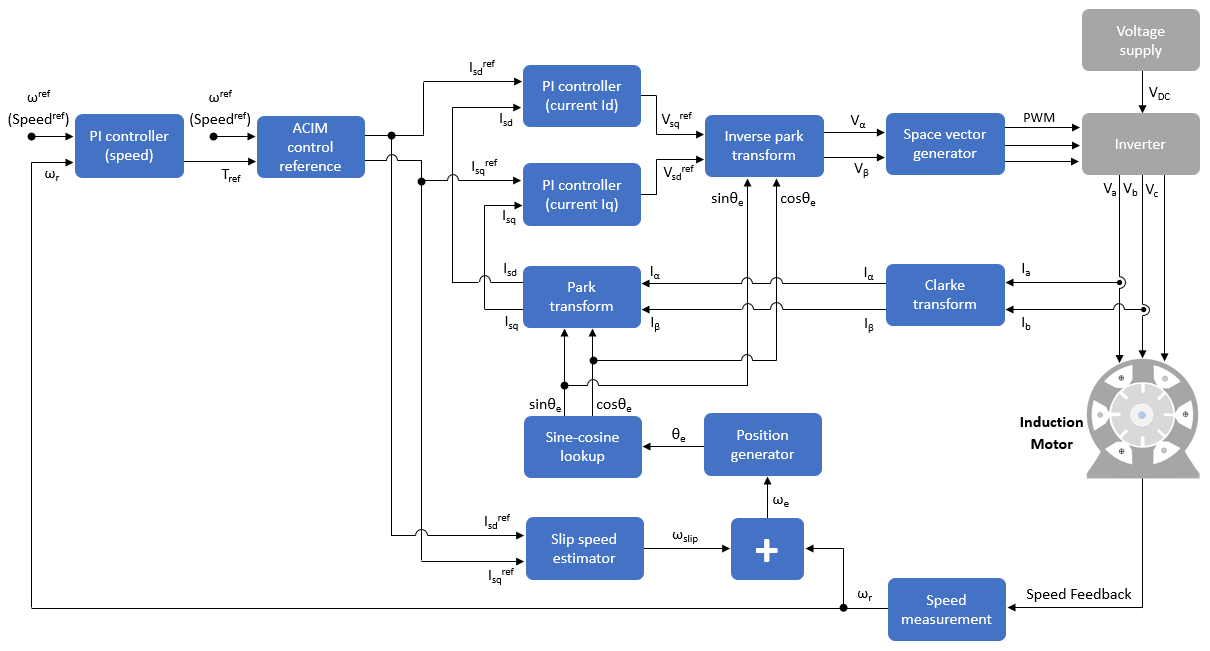
\includegraphics[width=4in]{sections/section2/images/blockDiagram.png}}

	\end{figure}
\end{frame}

% Slide 3: Block Diagram of the System
\begin{frame}{Block Diagram of the System}
	\begin{figure}
		\centering

		\fbox{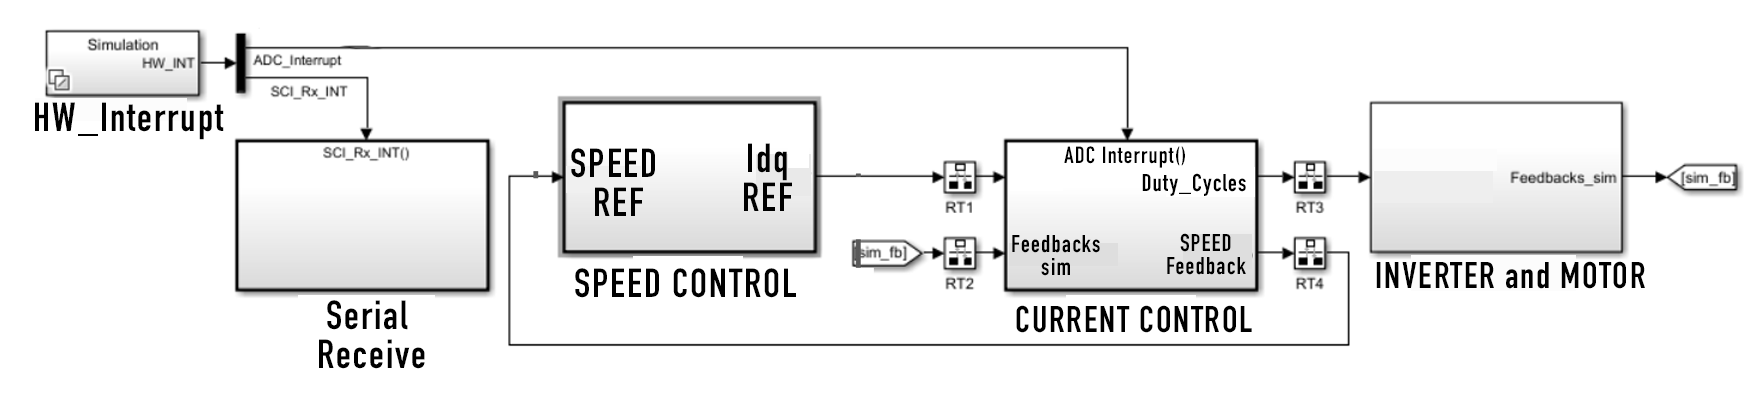
\includegraphics[width=4in]{sections/section3/images/simulation/blockDia.png}}

	\end{figure}
\end{frame}

% Slide 4: Speed Control Subsystem
\begin{frame}{Speed Control Subsystem}
	\begin{figure}
		\centering

		\fbox{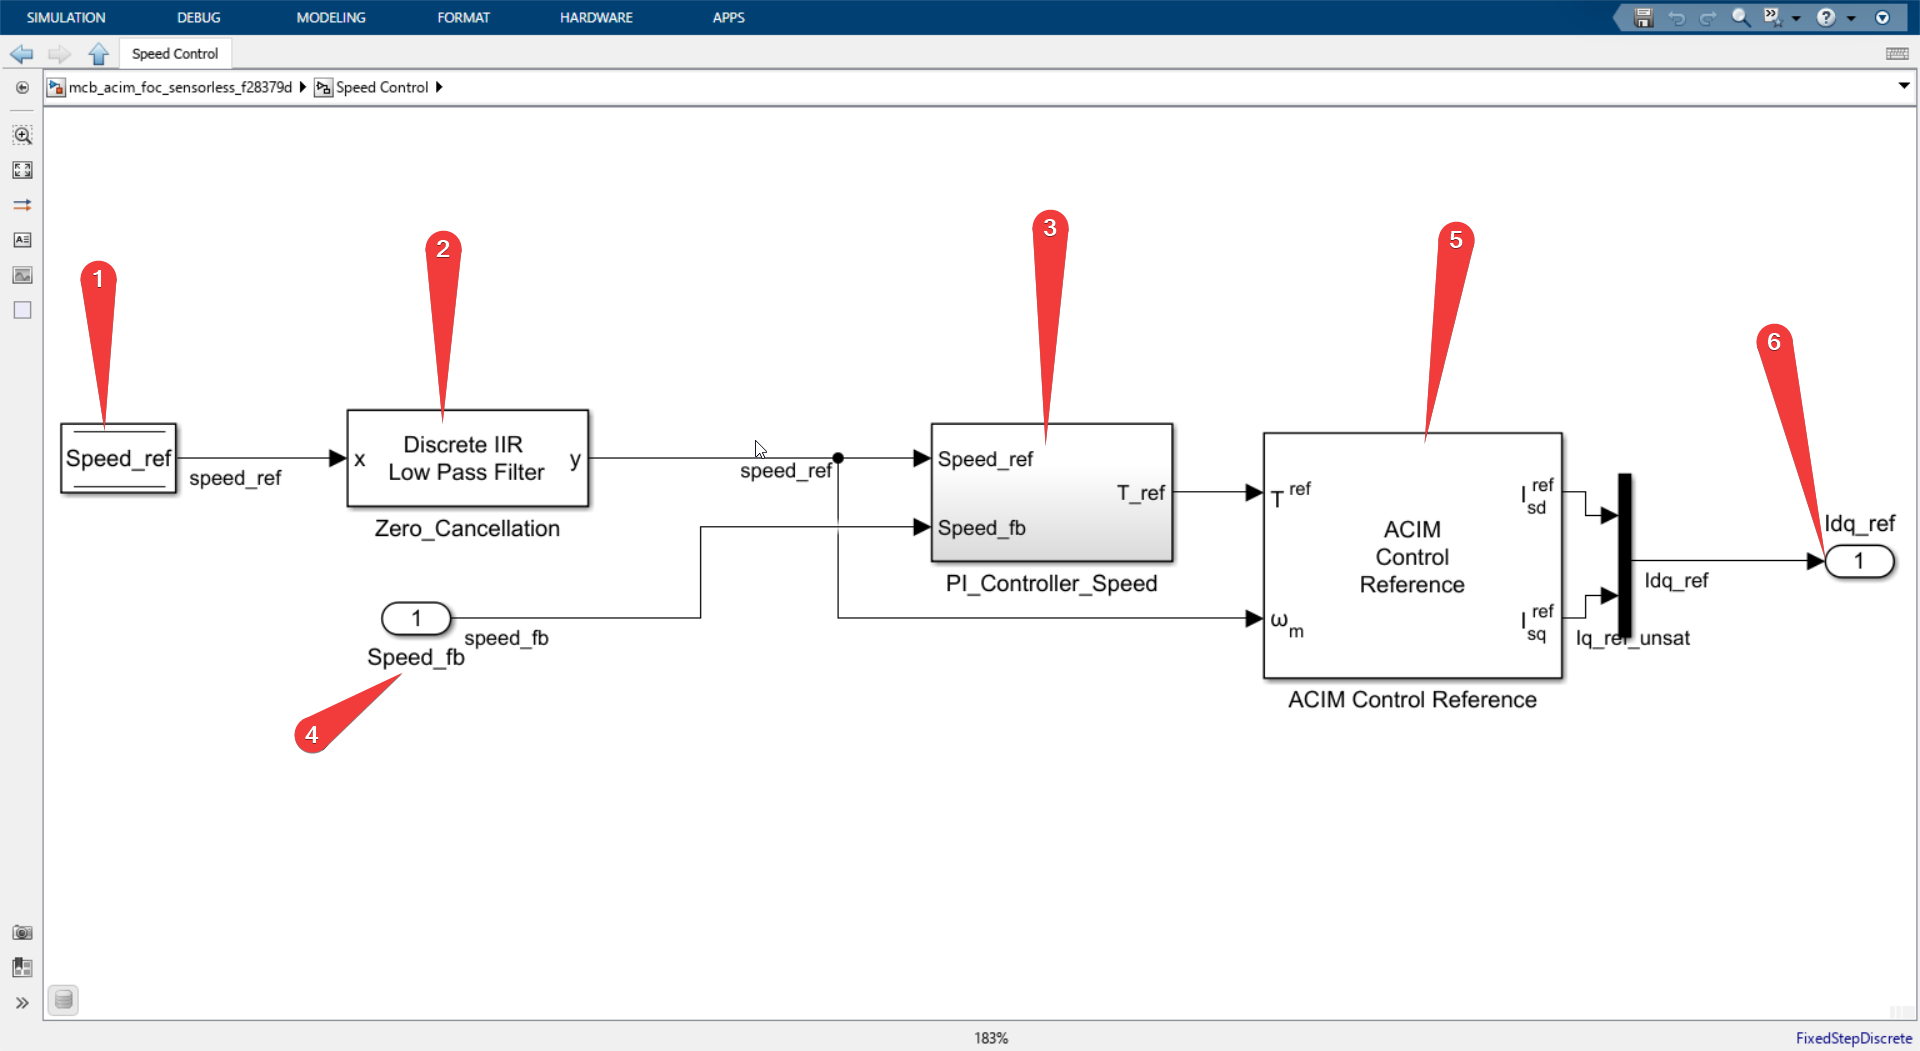
\includegraphics[width=4in]{sections/section3/images/simulation/speedControl/speedController.png}}

	\end{figure}
\end{frame}

% Slide 5: Current Measurement
\begin{frame}{Current Measurement}
	\begin{figure}
		\centering

		\fbox{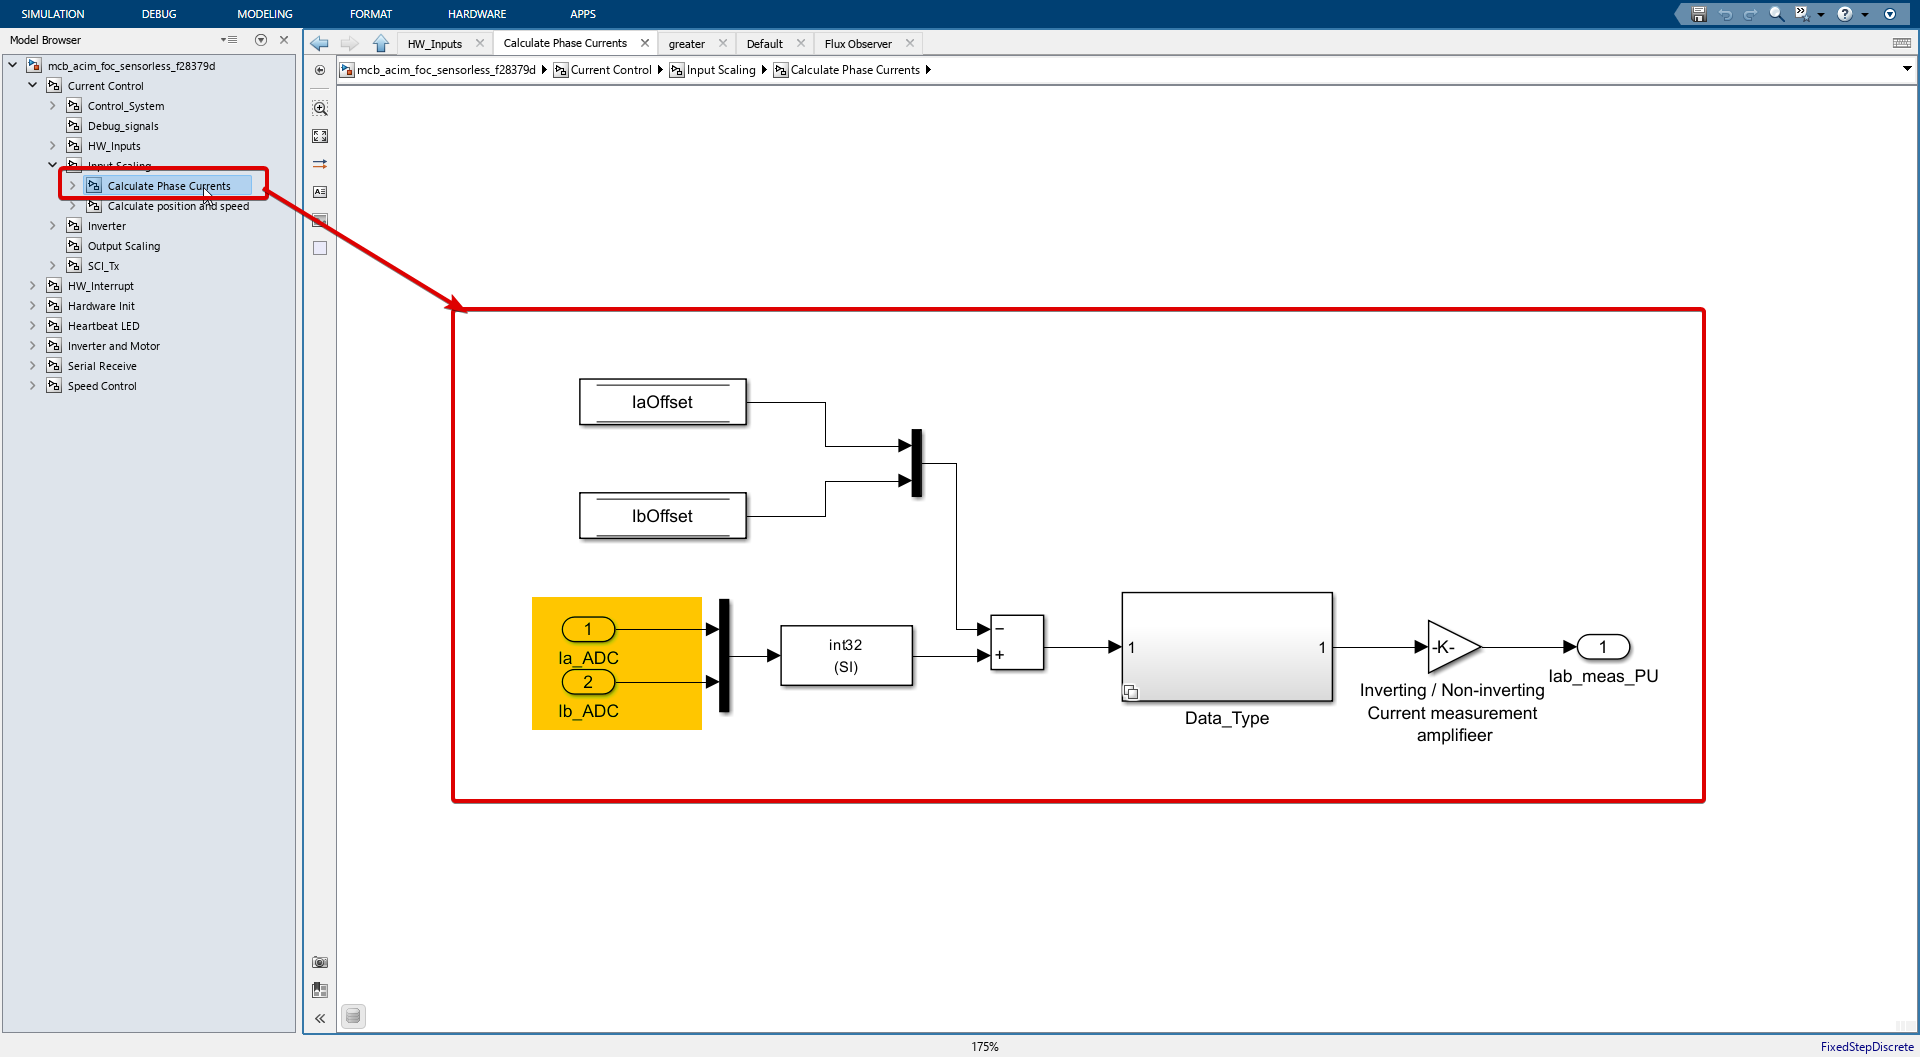
\includegraphics[width=4in]{sections/section3/images/simulation/inputScaling/currentMeasurement.png}}

	\end{figure}
\end{frame}

% Slide 6: Position and Speed Estimation
\begin{frame}{Position and Speed Estimation}
	\begin{figure}
		\centering

		\fbox{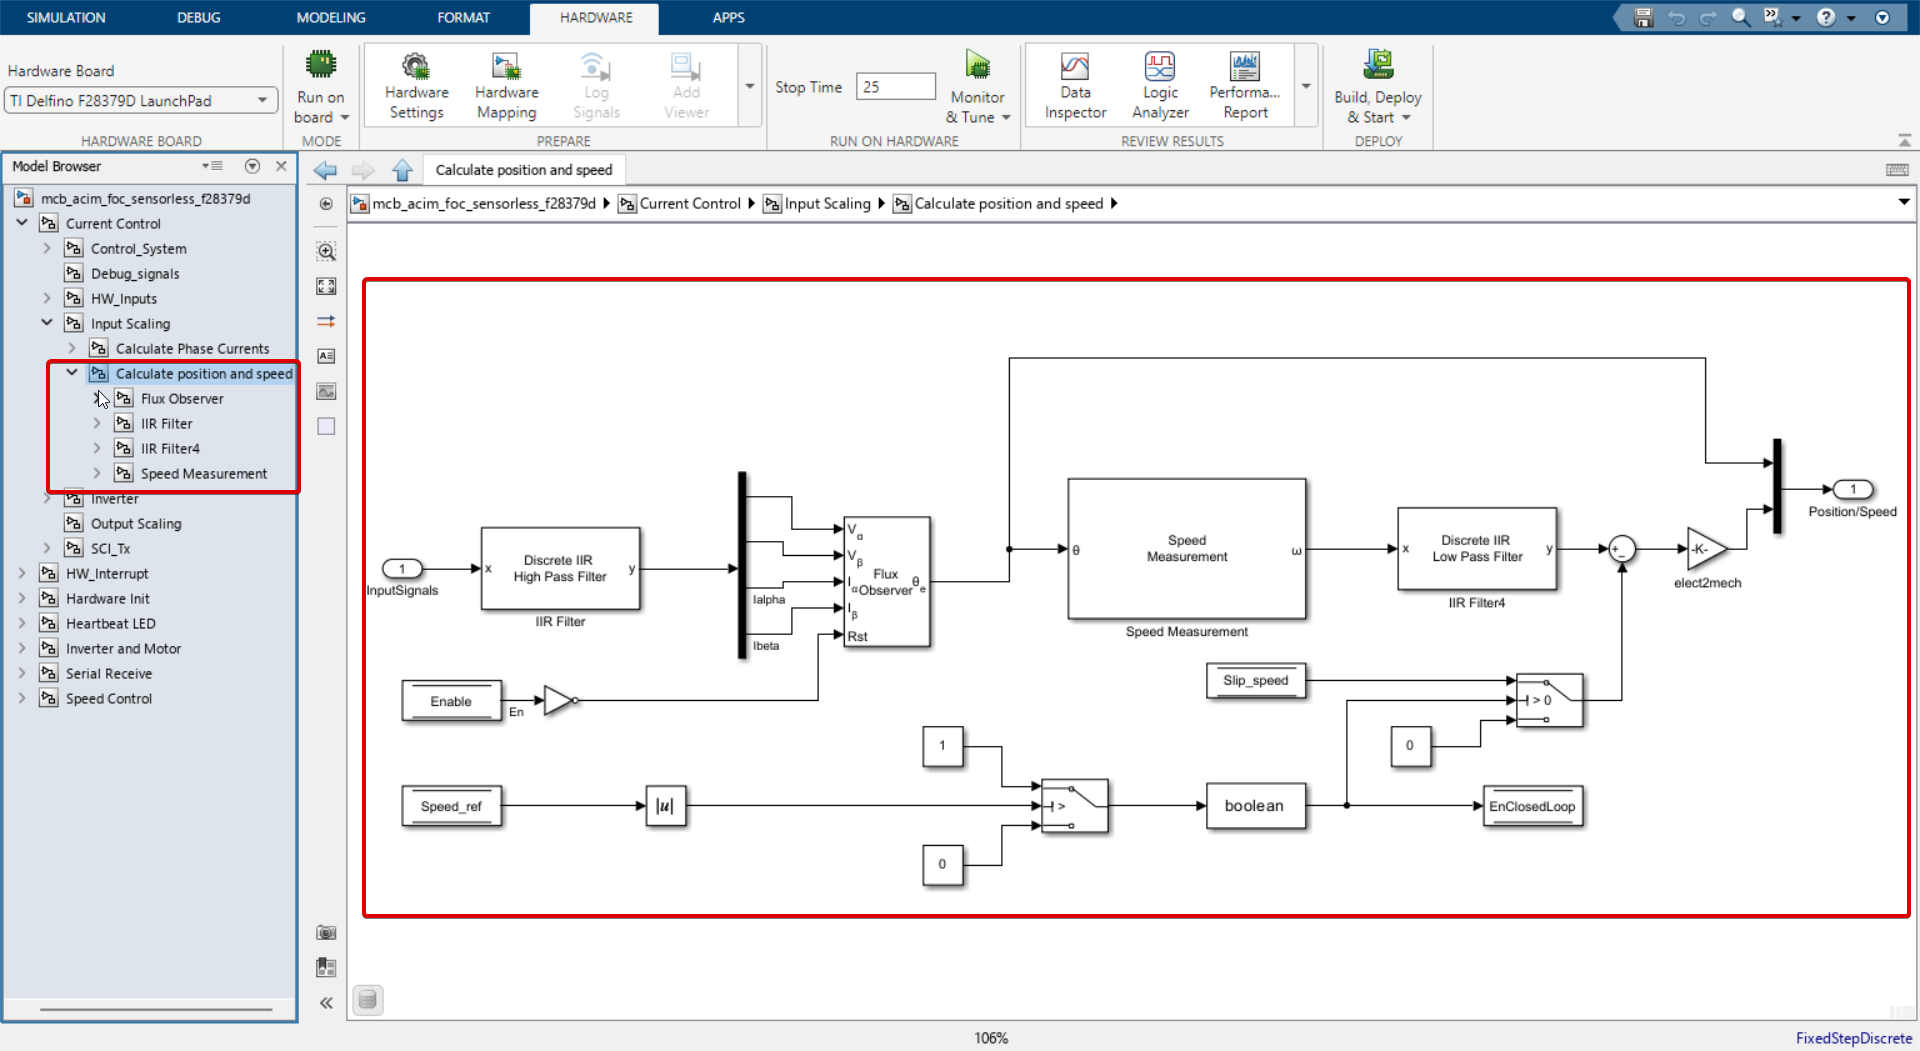
\includegraphics[width=4in]{sections/section3/images/simulation/inputScaling/fluxObserver.png}}

	\end{figure}
\end{frame}

% Slide 7: Current Control System
\begin{frame}{Current Control System}
	\begin{figure}
		\centering

		\fbox{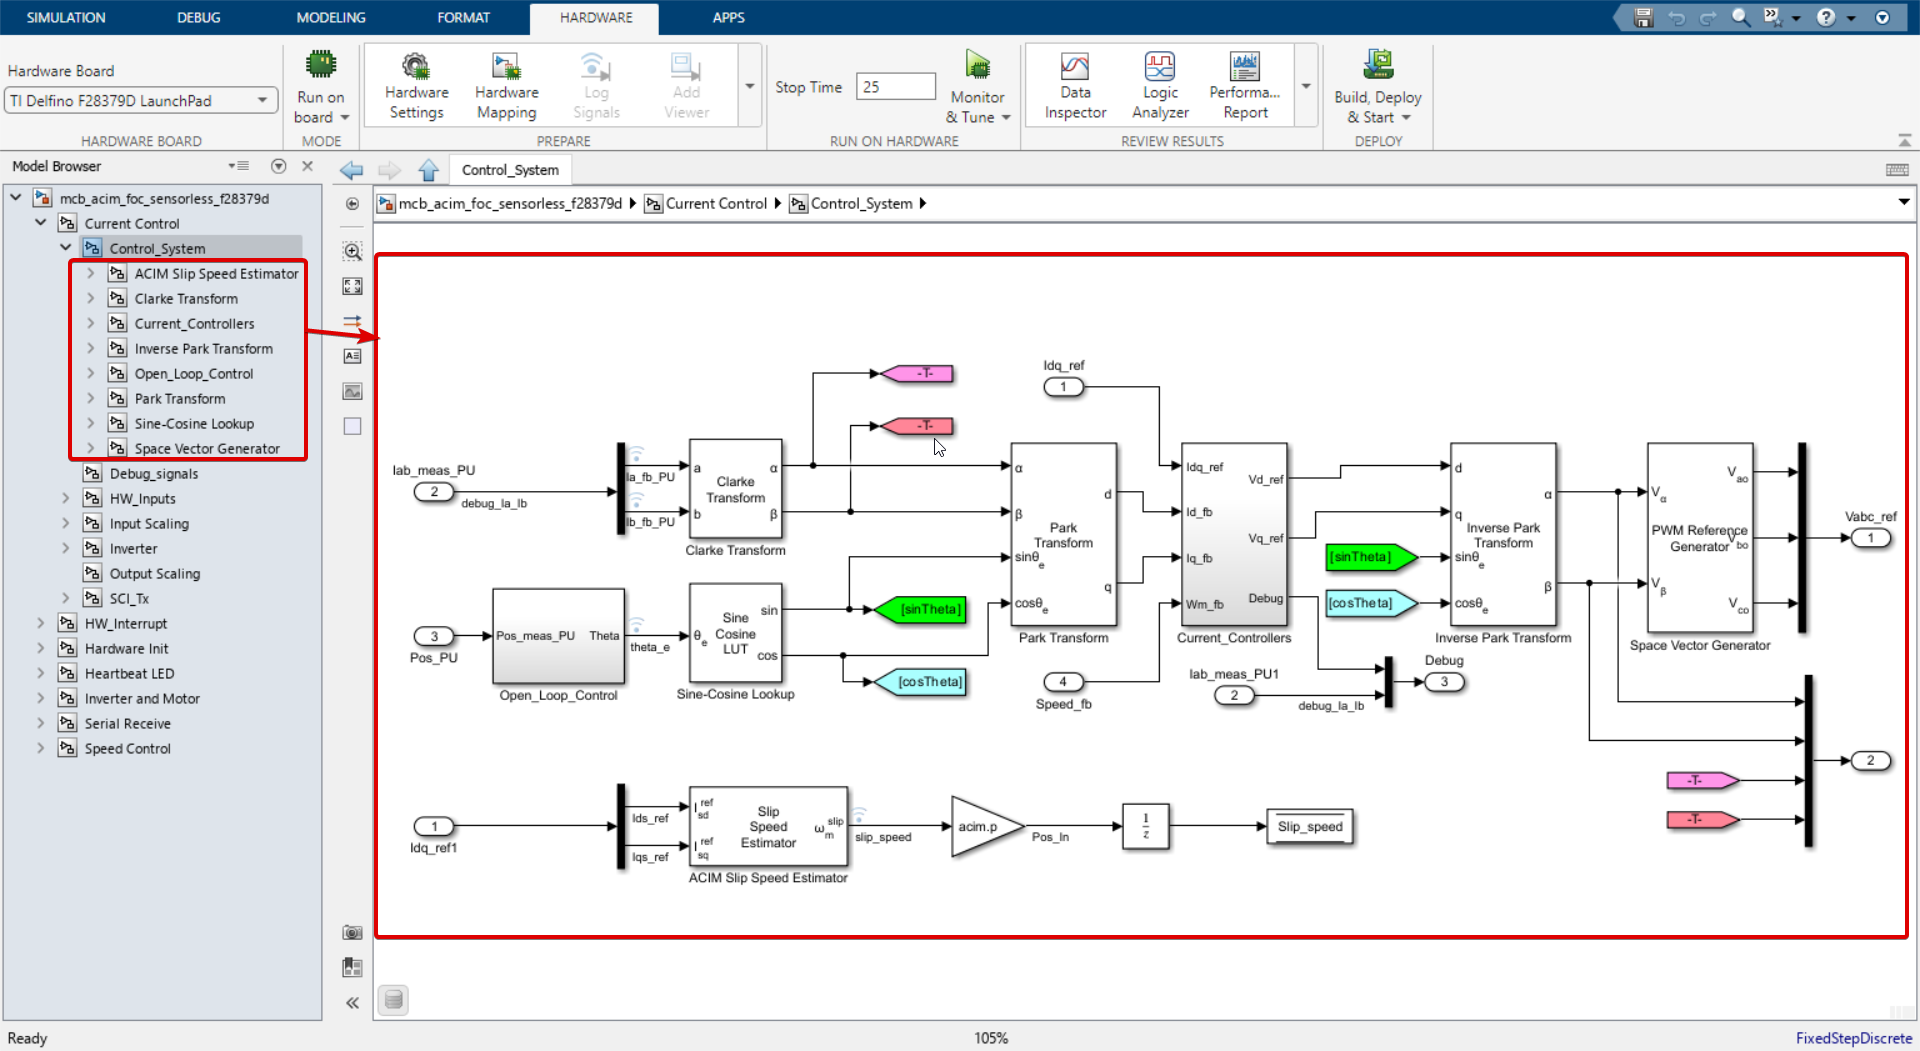
\includegraphics[width=4in]{sections/section3/images/simulation/currentControl/controlSystem.png}}

	\end{figure}
\end{frame}

% Slide 8: Speed Response
\begin{frame}{Speed Response}
	\begin{figure}
		\centering

		\fbox{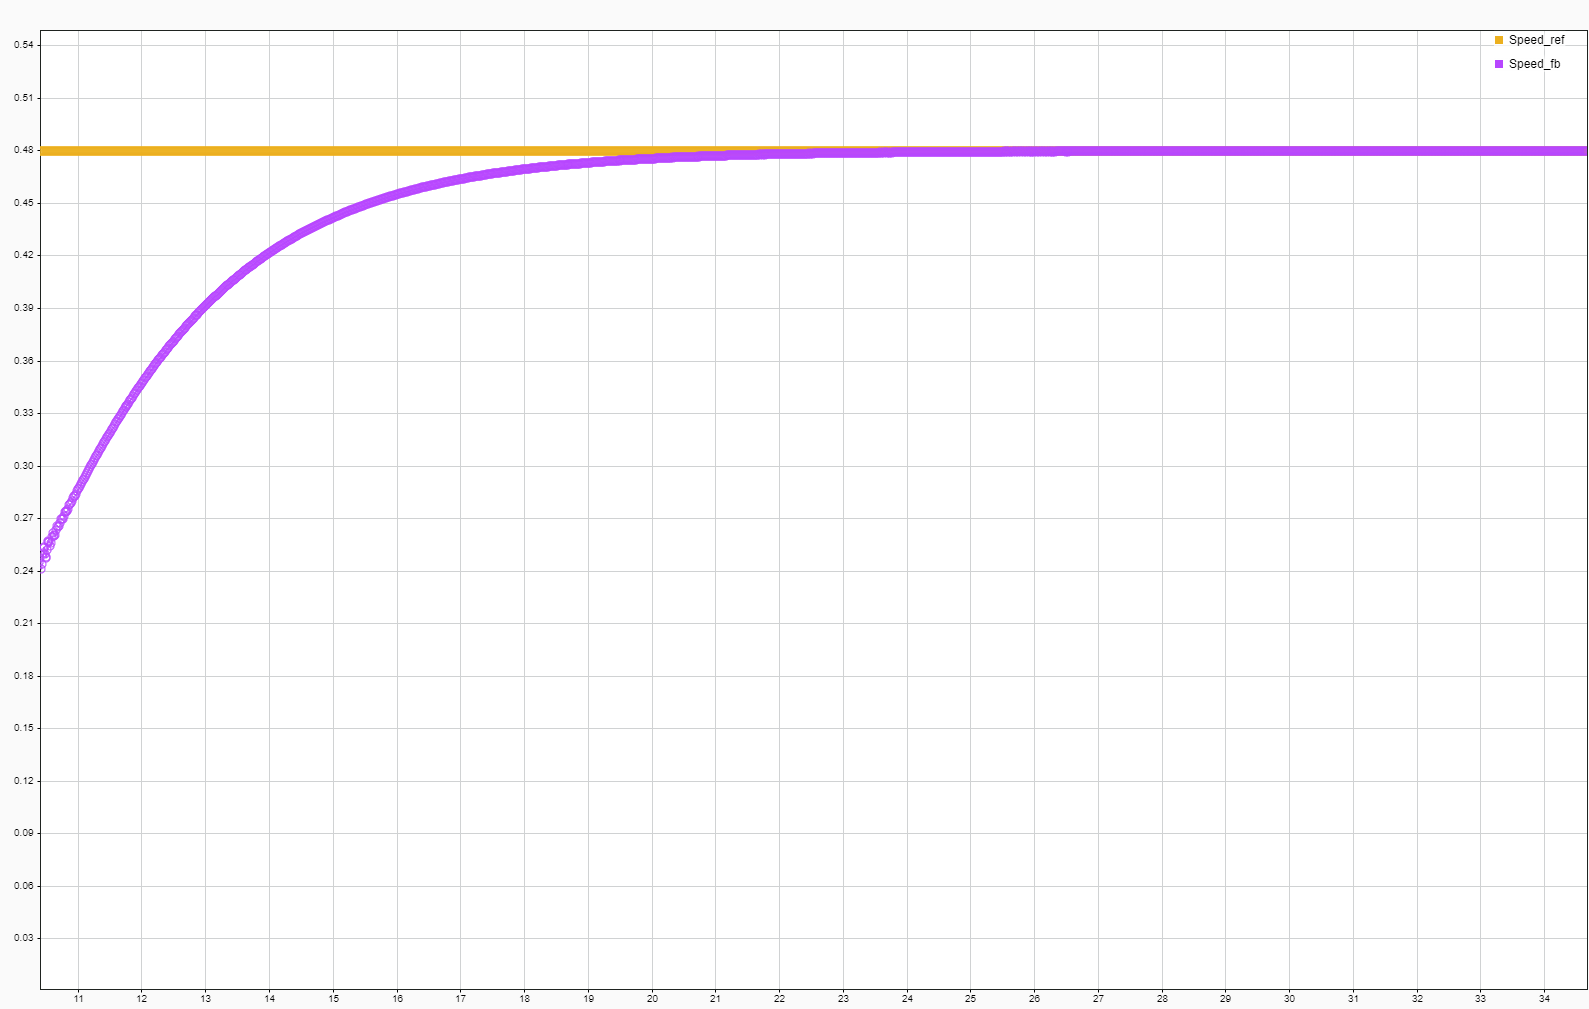
\includegraphics[width=4in]{sections/section3/images/simulationResutls/SpeedTrackingNoCursor.png}}

	\end{figure}
\end{frame}

% Slide 9: Slip Speed
\begin{frame}{Slip Speed}
	\begin{figure}
		\centering

		\fbox{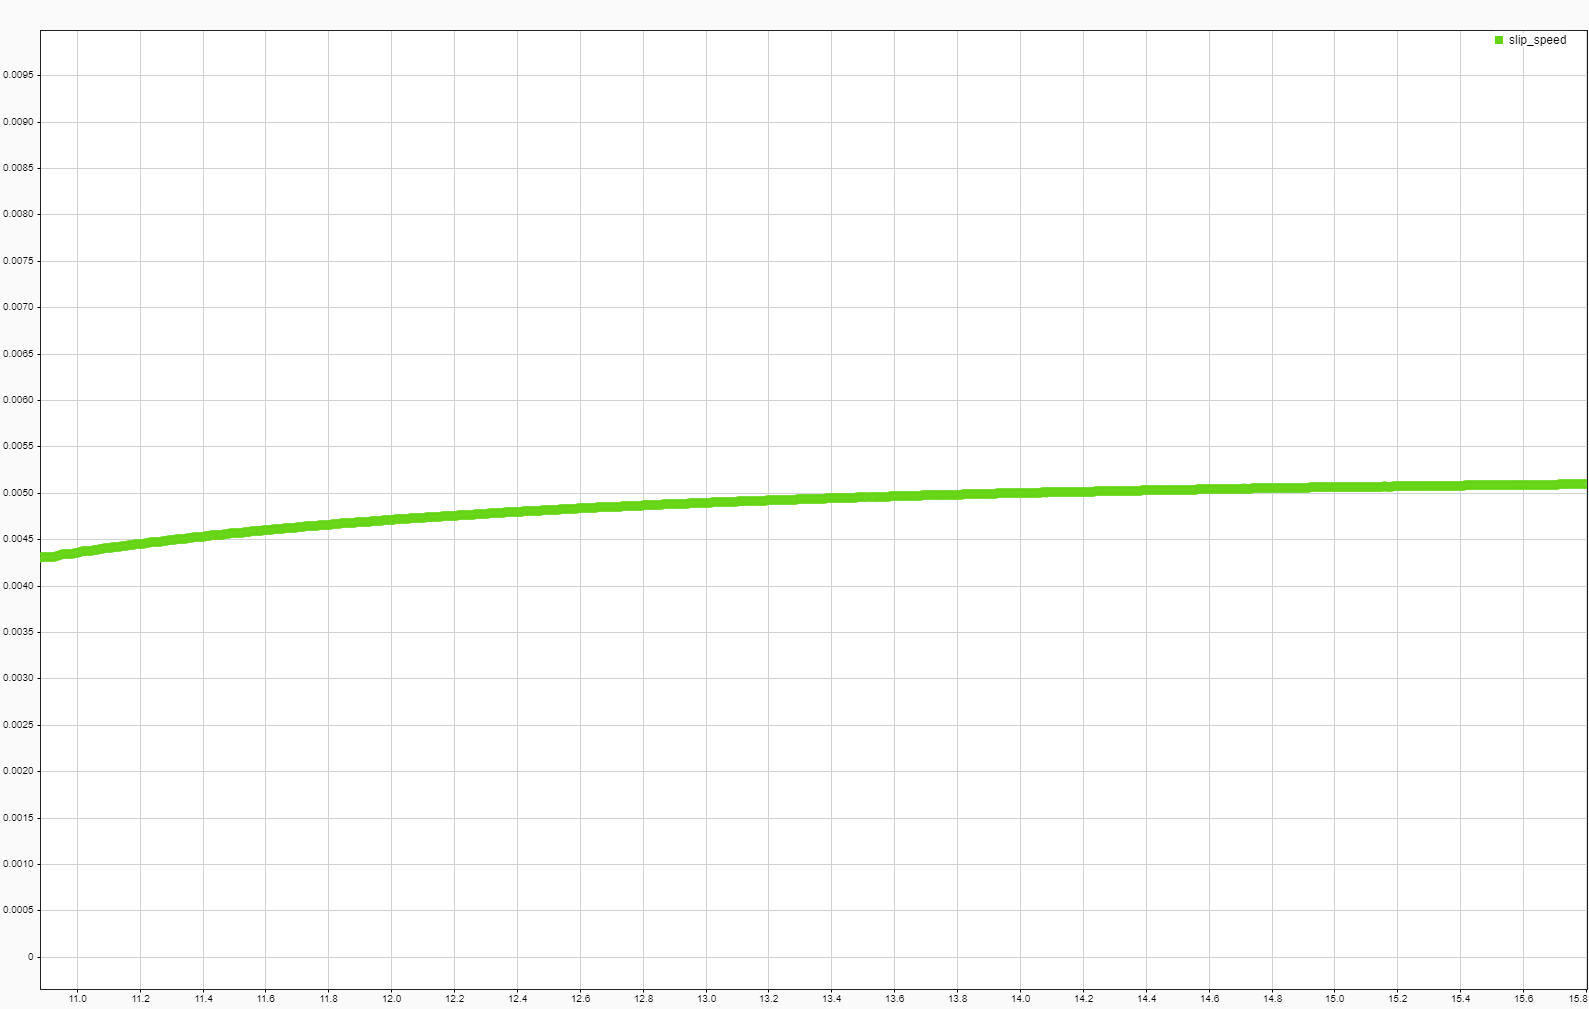
\includegraphics[width=4in]{sections/section3/images/simulationResutls/SlipSpeed.png}}

	\end{figure}
\end{frame}

% ... (previous slides)

% Slide 10: Ia and Ib Feedback/Measured Currents
\begin{frame}{Ia and Ib Feedback/Measured Currents}
	\begin{figure}
		\centering

		\fbox{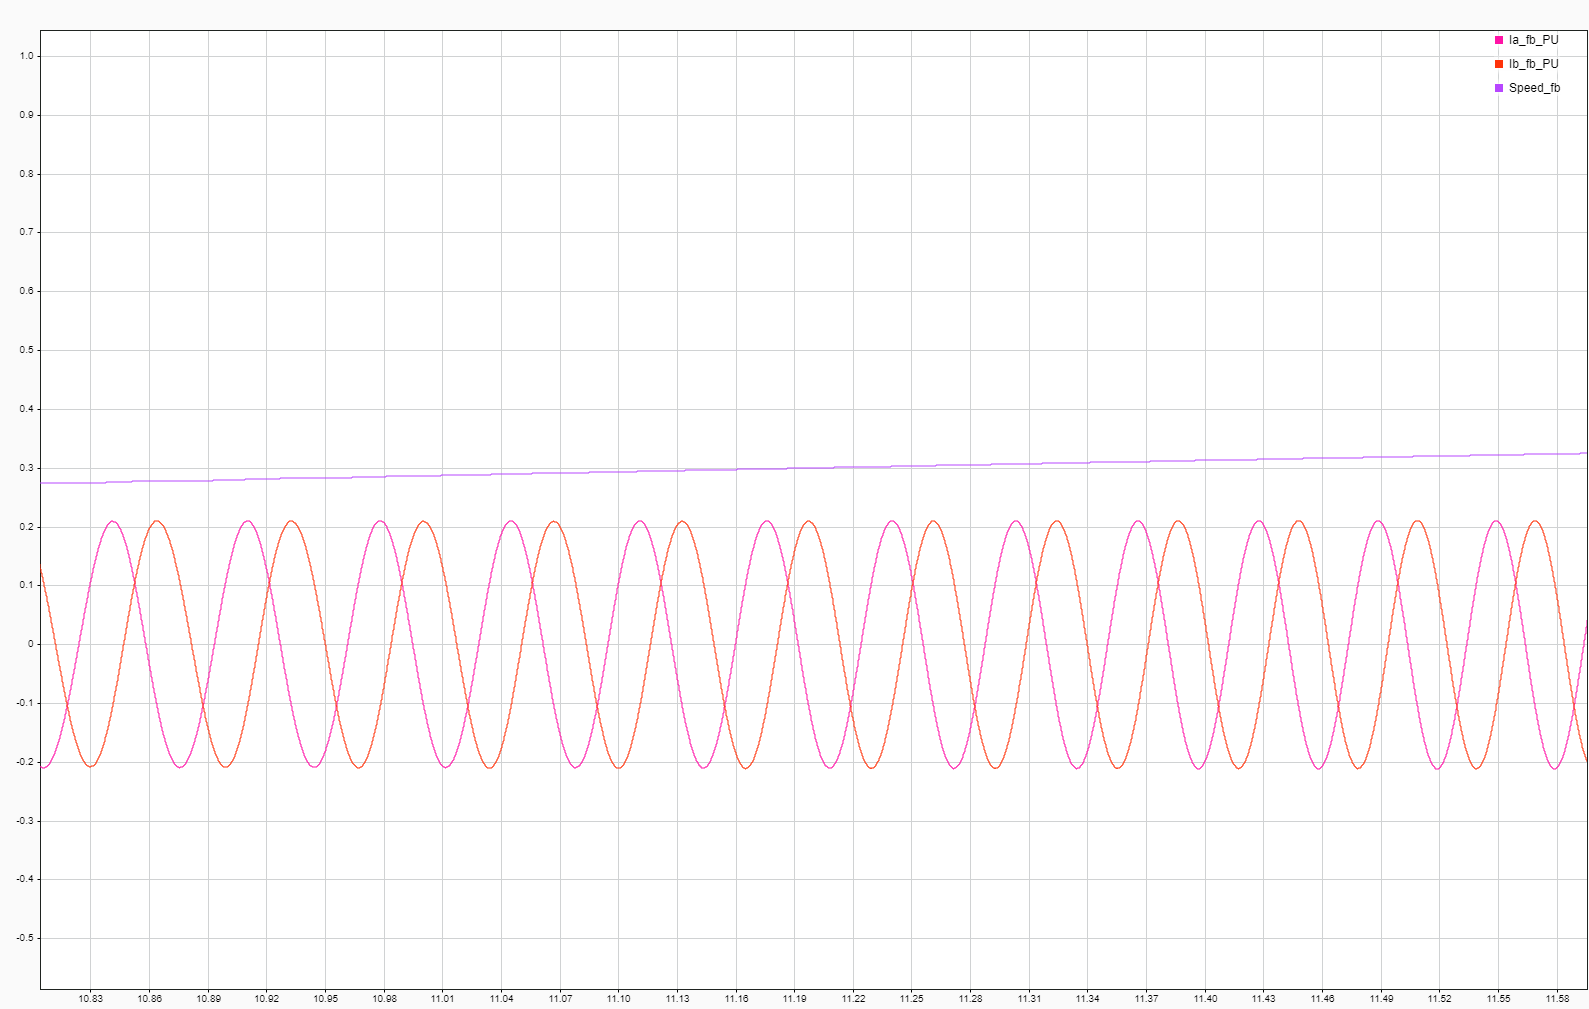
\includegraphics[width=4in]{sections/section3/images/simulationResutls/Ia_Ib_fb.png}}

	\end{figure}
\end{frame}

% Slide 11: Id and Iq Reference Currents
\begin{frame}{Id and Iq Reference Currents}
	\begin{figure}
		\centering

		\fbox{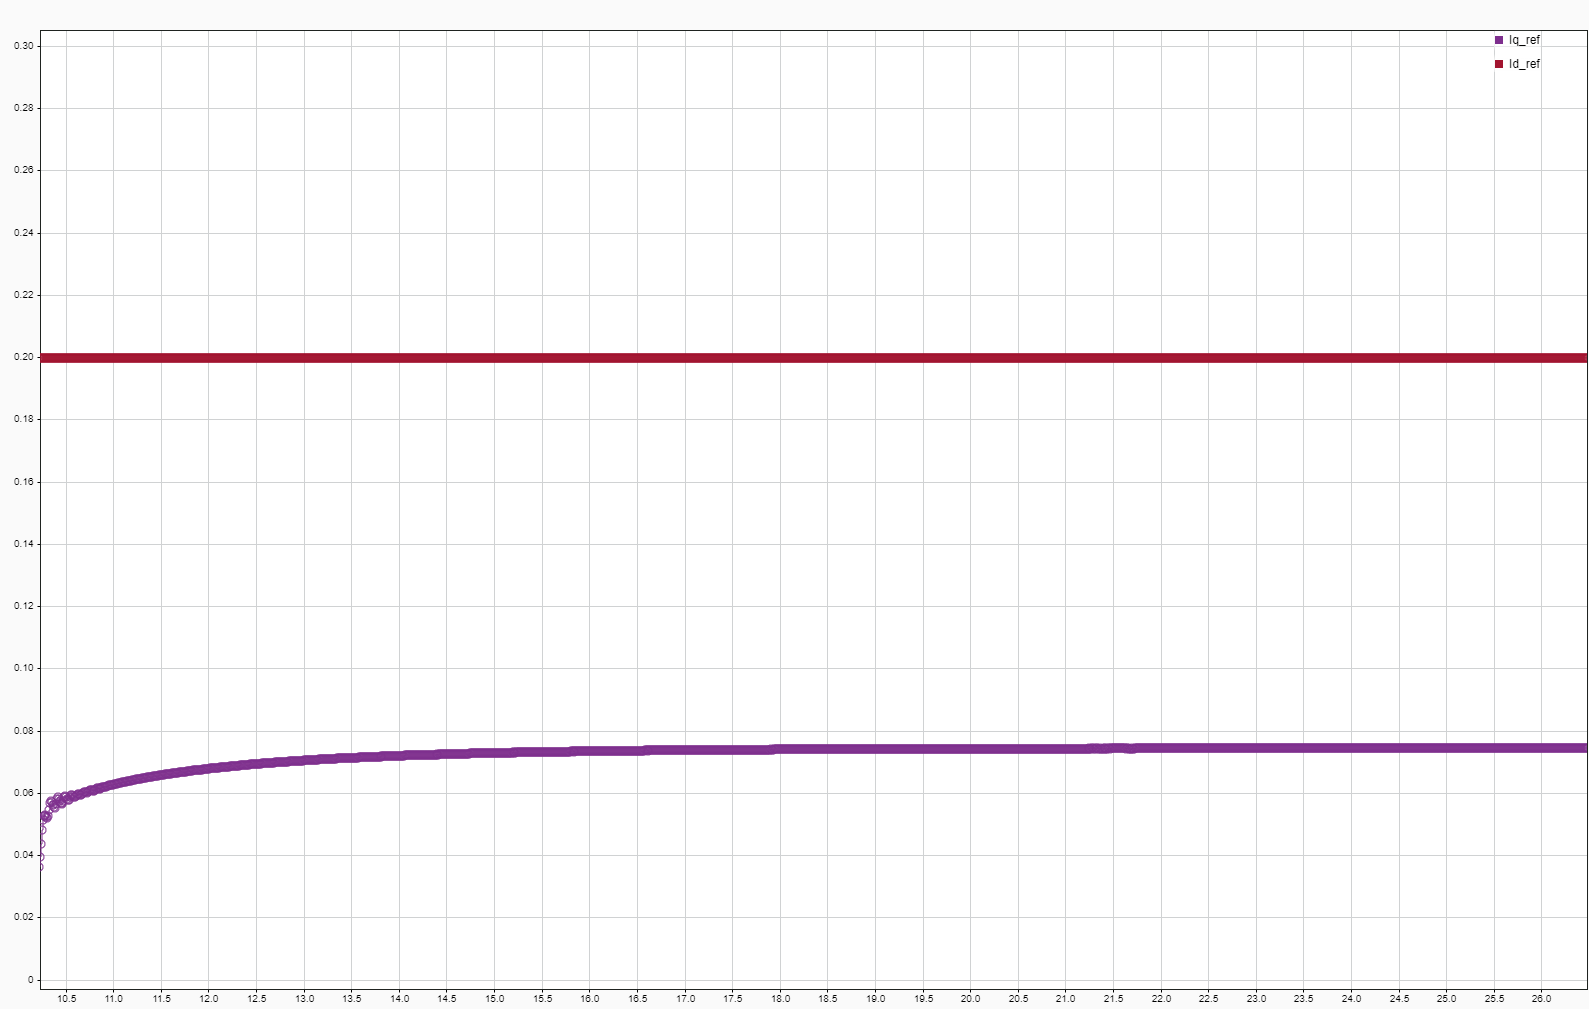
\includegraphics[width=4in]{sections/section3/images/simulationResutls/Id_ref_Iq_ref.png}}

	\end{figure}
\end{frame}

% Slide 12: Id and Iq Feedback Currents
\begin{frame}{Id and Iq Feedback Currents}
	\begin{figure}
		\centering

		\fbox{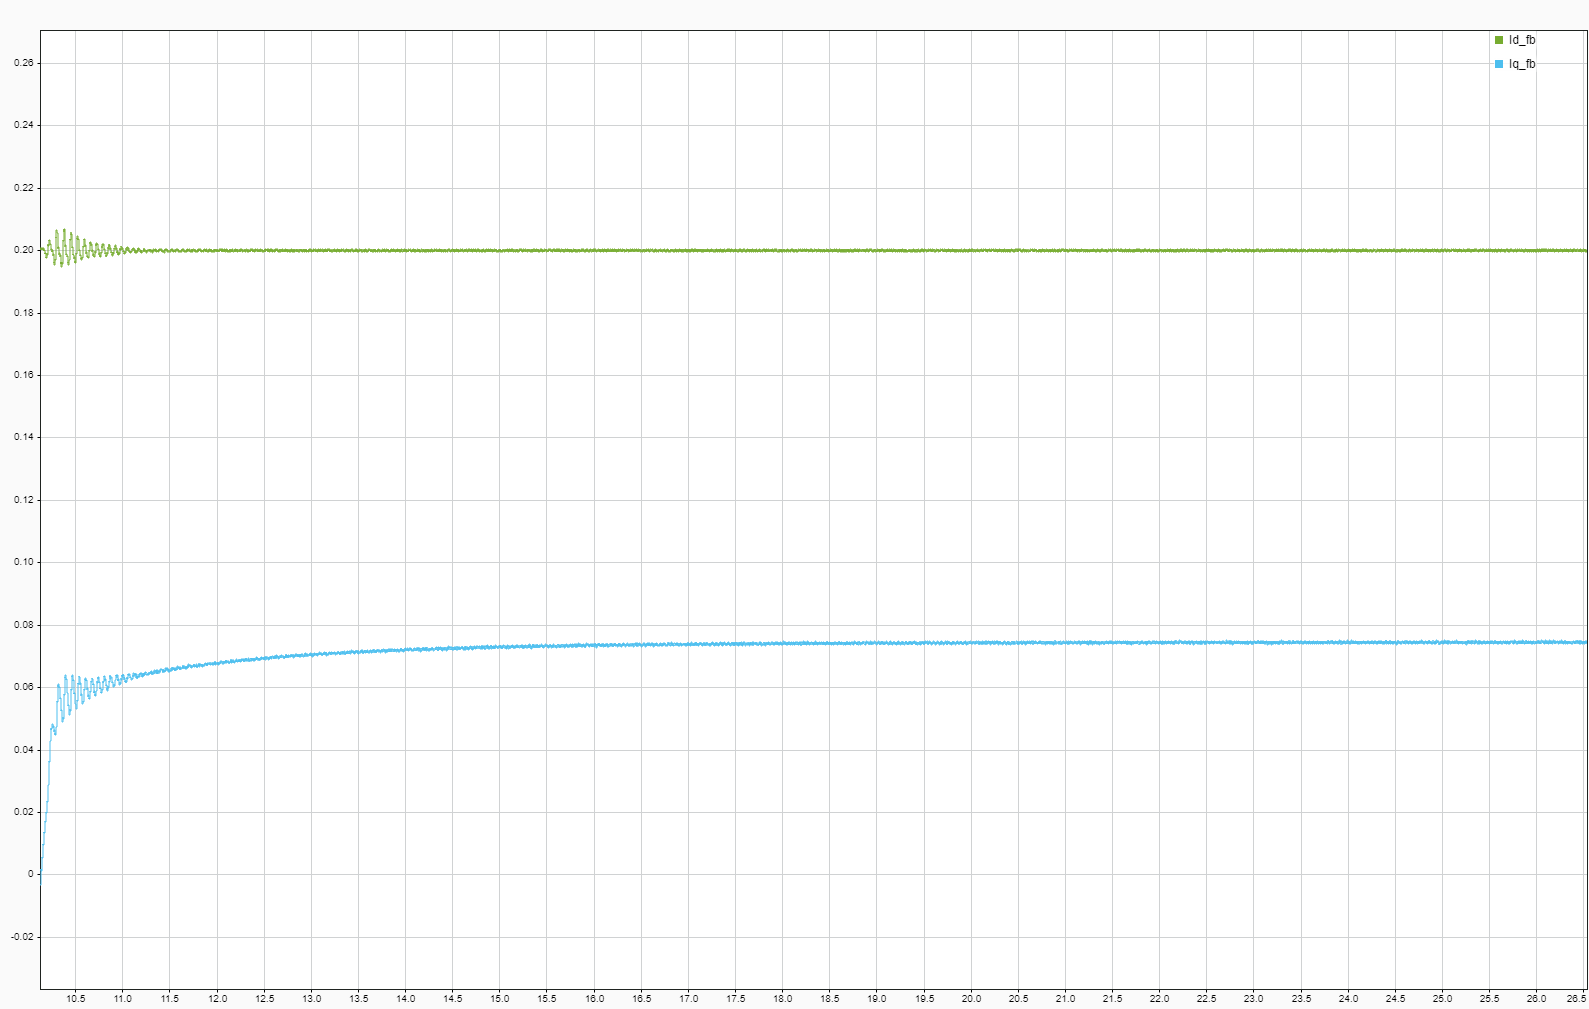
\includegraphics[width=4in]{sections/section3/images/simulationResutls/Id_fb_Iq_fb.png}}

	\end{figure}
\end{frame}

% Slide 13: Iq Reference and Feedback Currents (Torque producing current)
\begin{frame}{Iq Reference and Feedback Currents (Torque producing current)}
	\begin{figure}
		\centering

		\fbox{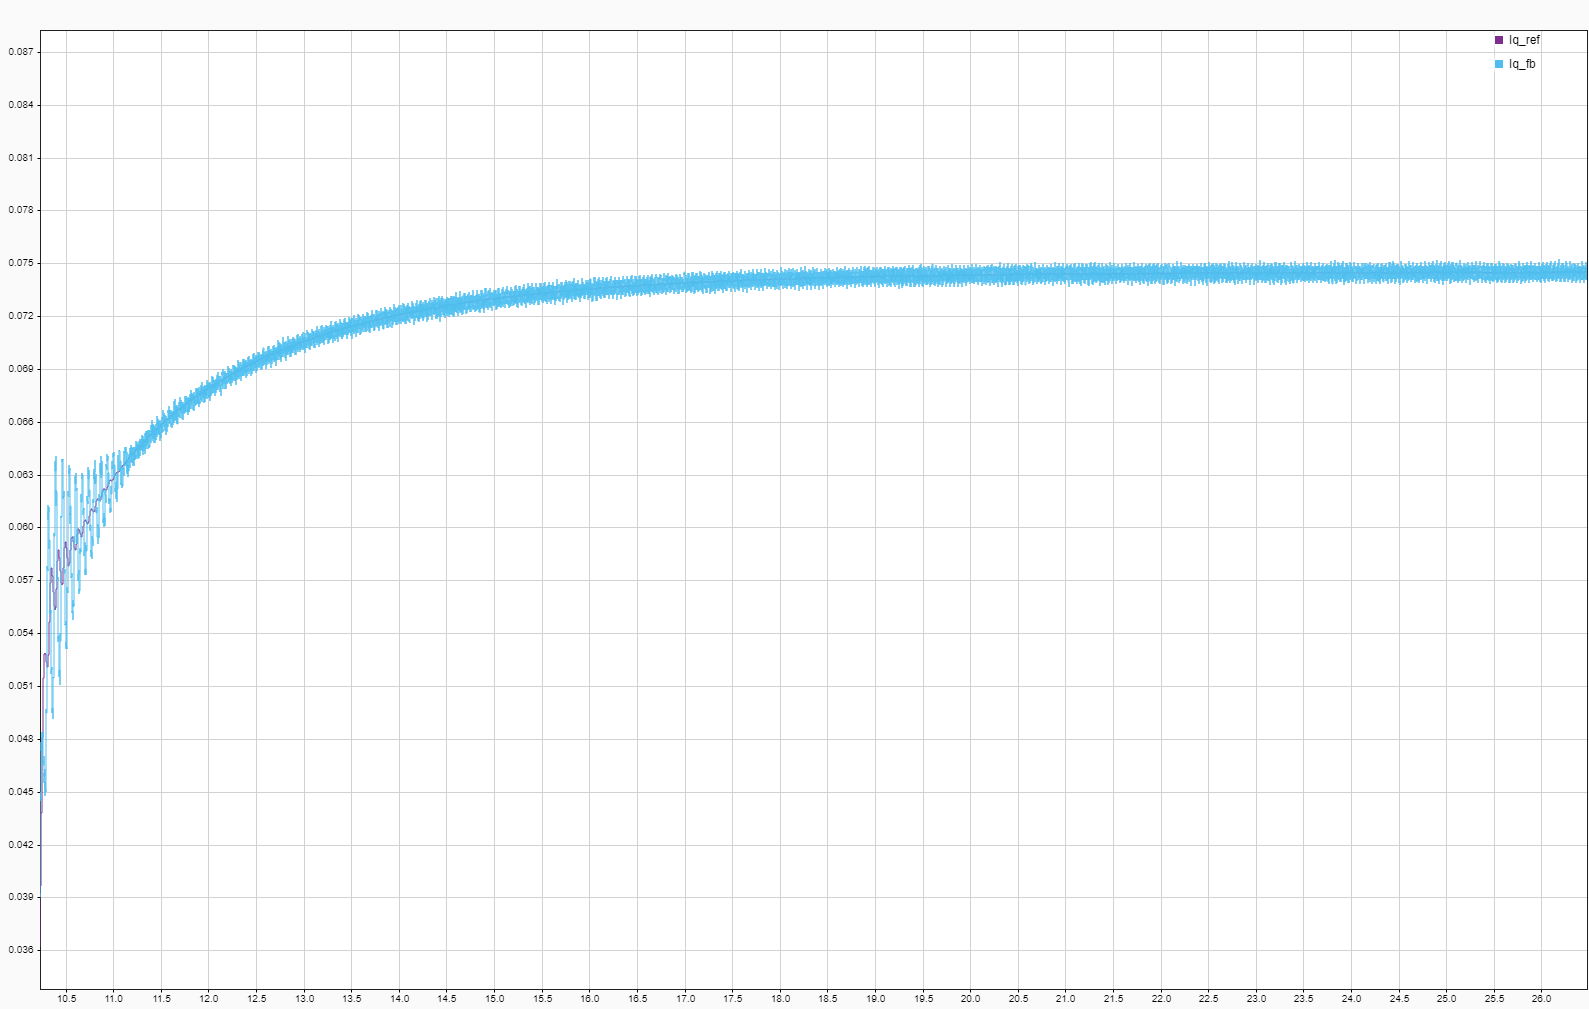
\includegraphics[width=4in]{sections/section3/images/simulationResutls/Iq_ref_fb.png}}

	\end{figure}
\end{frame}

% Slide 14: Id Reference and Feedback Currents (Magnetizing current)
\begin{frame}{Id Reference and Feedback Currents (Magnetizing current)}
	\begin{figure}
		\centering

		\fbox{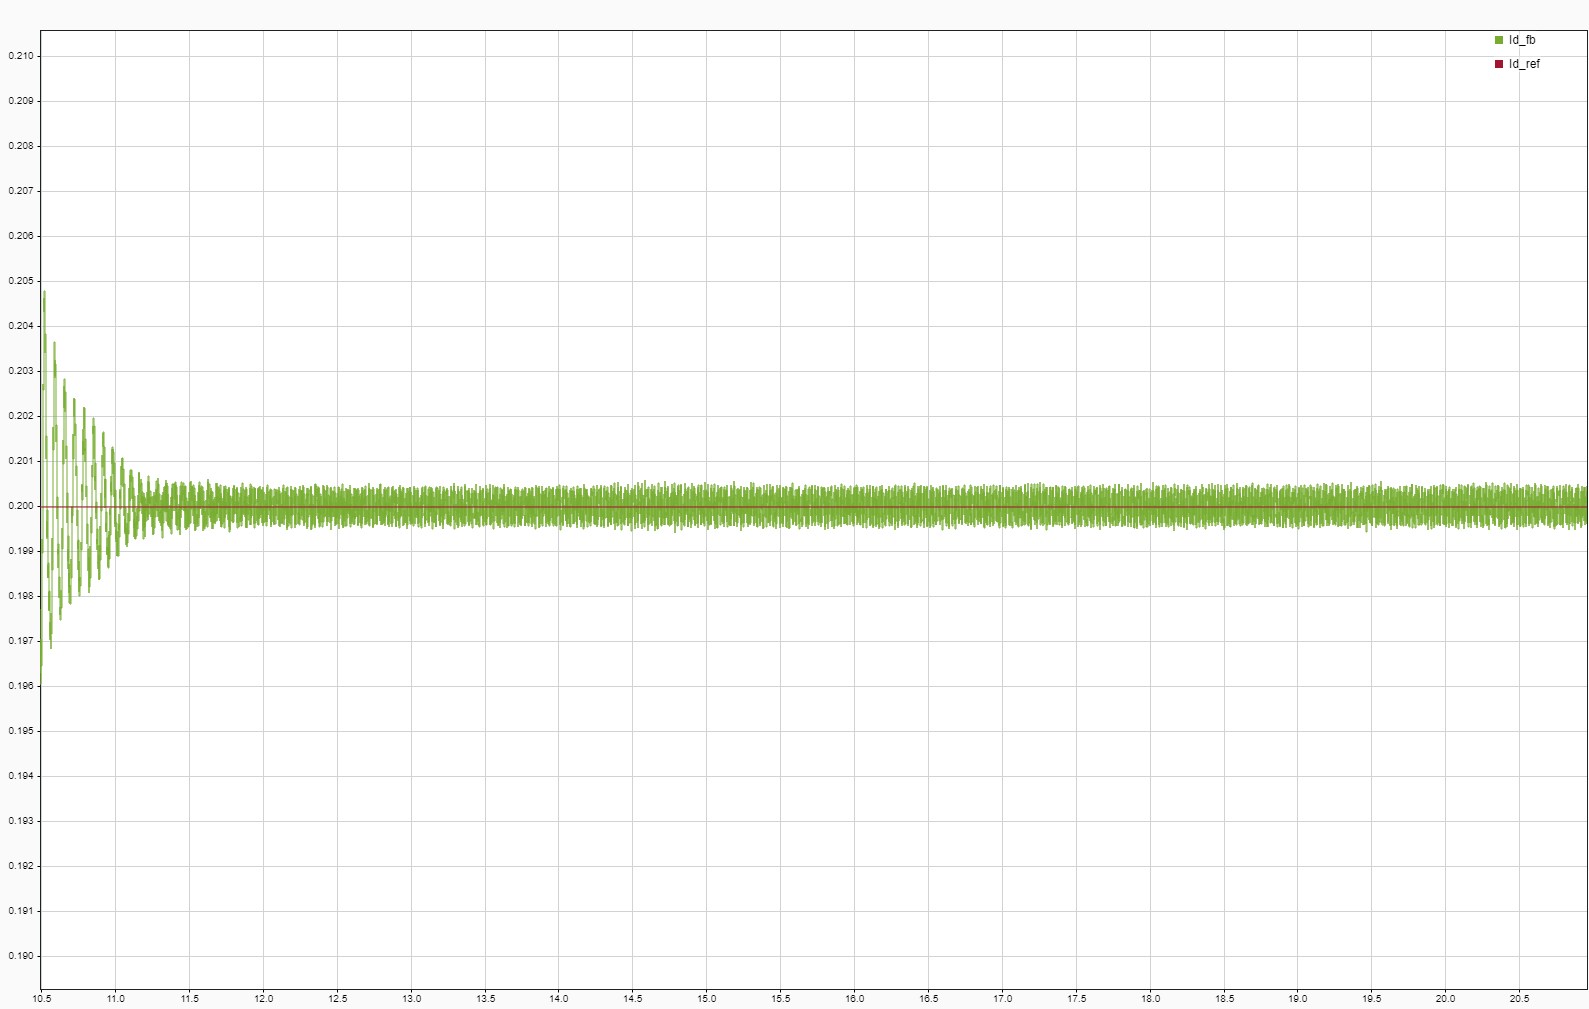
\includegraphics[width=4in]{sections/section3/images/simulationResutls/Id_ref_fb.png}}

	\end{figure}
\end{frame}

% Slide 15: Image of Induction Motor
\begin{frame}{Induction Motor}
	\begin{figure}
		\centering

		\fbox{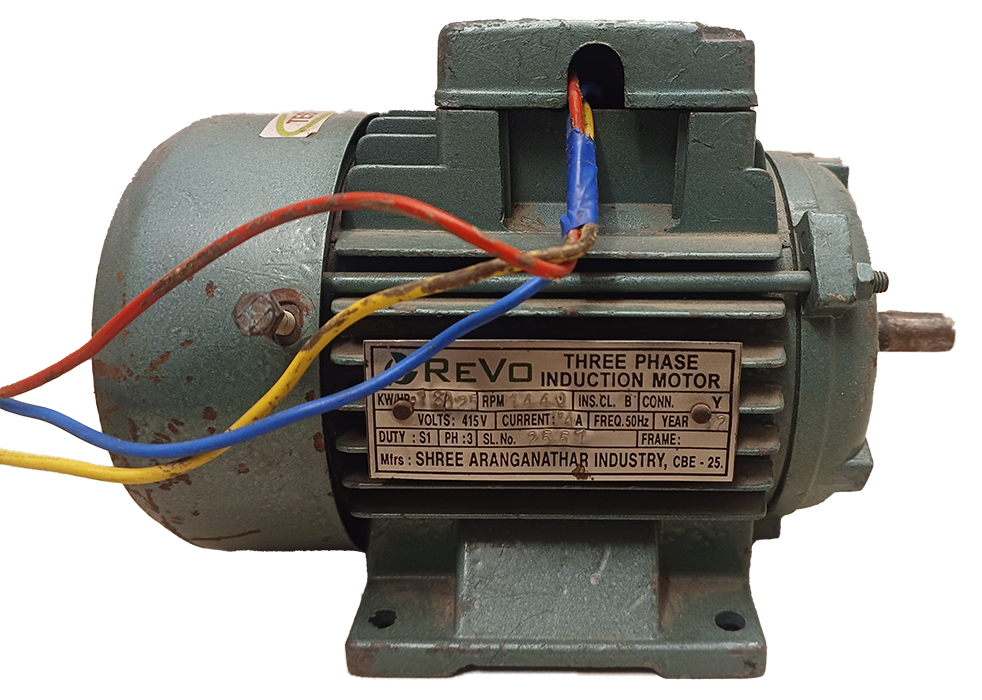
\includegraphics[width=4in]{sections/section4/images/inductionMotor/revo.png}}

	\end{figure}
\end{frame}

% Slide 16: Image of F28379D Launchpad
\begin{frame}{F23879d Launchpad}
	\begin{figure}
		\centering

		\fbox{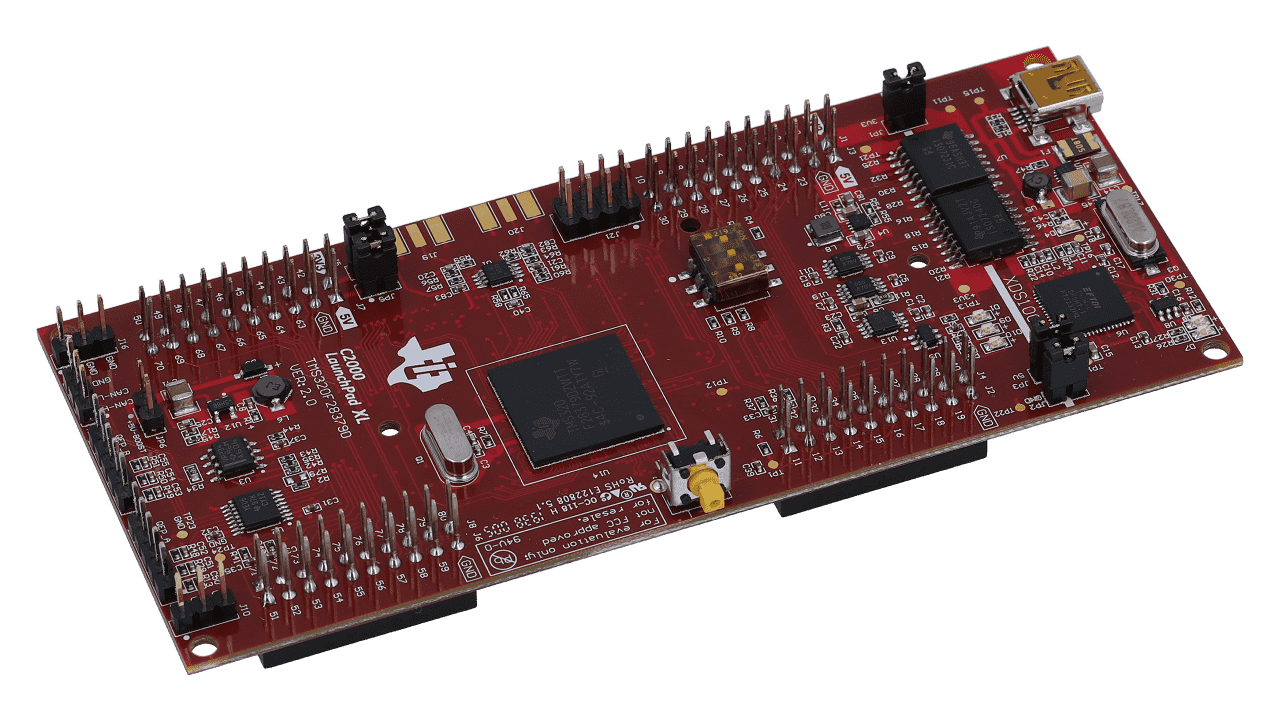
\includegraphics[width=4in]{sections/section4/images/f23879d/launchxl-f28379d-angled.png}}

	\end{figure}
\end{frame}

% Slide 17: Image of FSAM20SH60A module
\begin{frame}{Intelligent Power Module Fsam20sh60a}
	\begin{figure}
		\centering

		\fbox{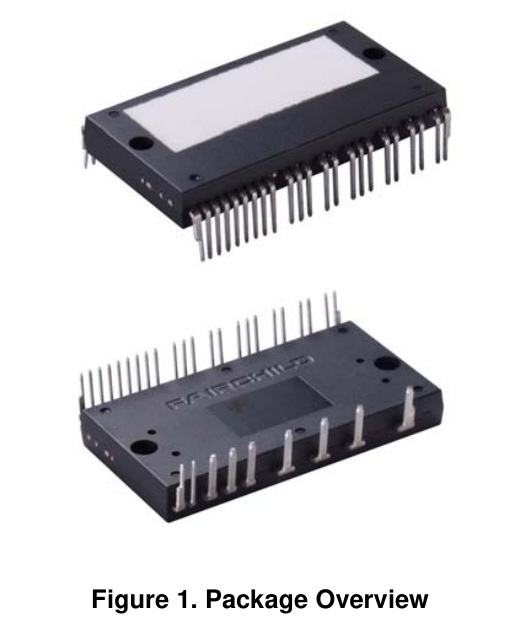
\includegraphics[width=4in]{sections/section4/images/IPM/ipm.png}}

	\end{figure}
\end{frame}

% Slide 18: Application Circuit from FSAM20SH60A Datasheet
\begin{frame}{PCB Design}
	\begin{figure}
		\centering

		\fbox{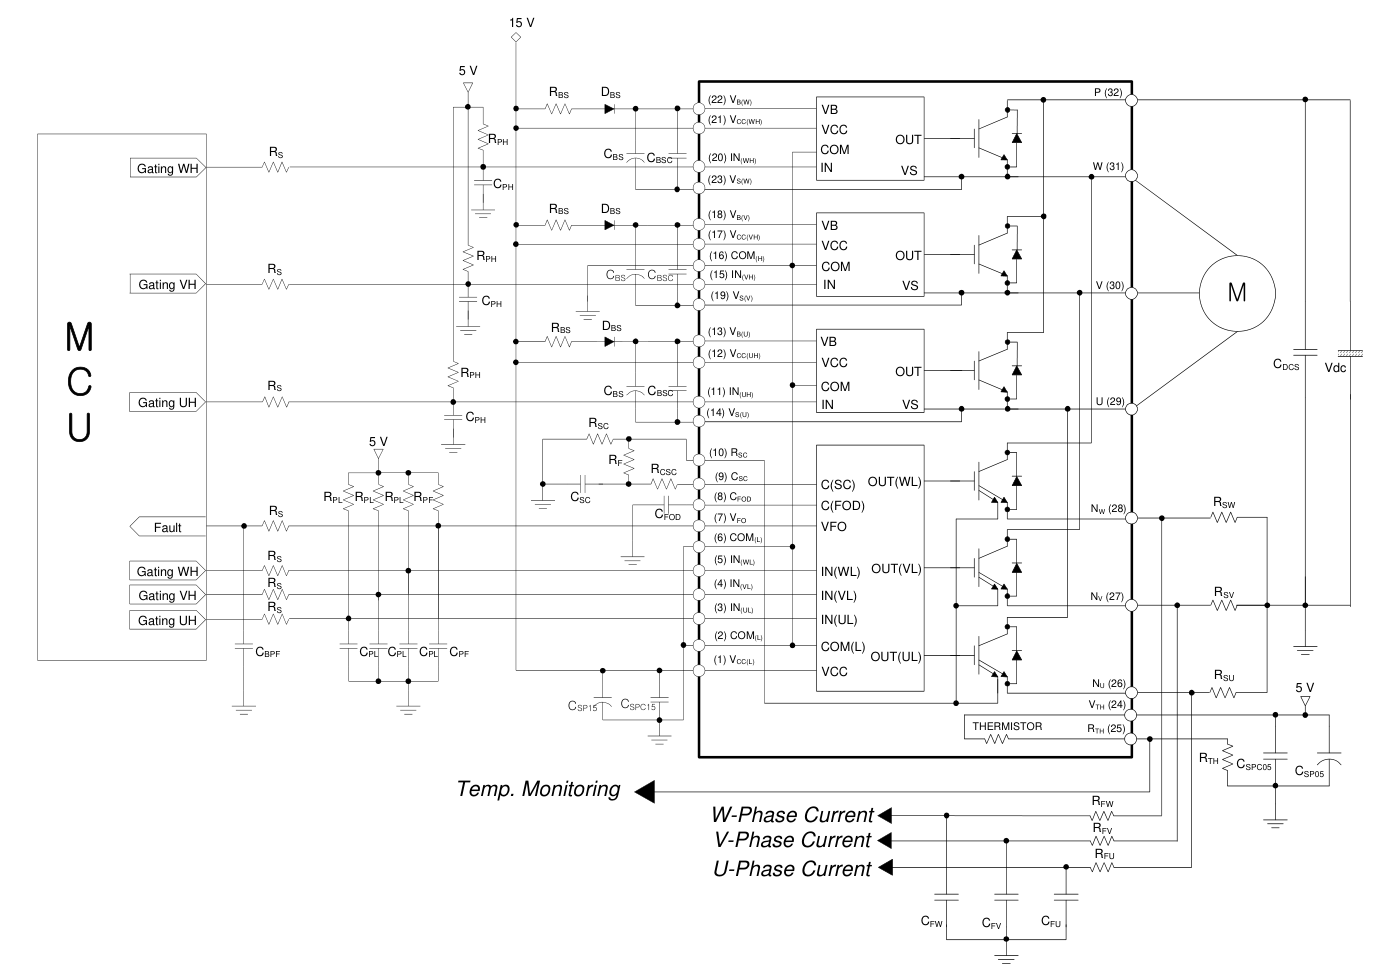
\includegraphics[width=4in]{sections/section4/images/PCBDesign/ApplicationCircuitfromDatasheet.png}}

	\end{figure}
\end{frame}

% Slide 19: PCB Layout Design in Ultiboard
\begin{frame}{PCB Layout Design}
	\begin{figure}
		\centering

		\fbox{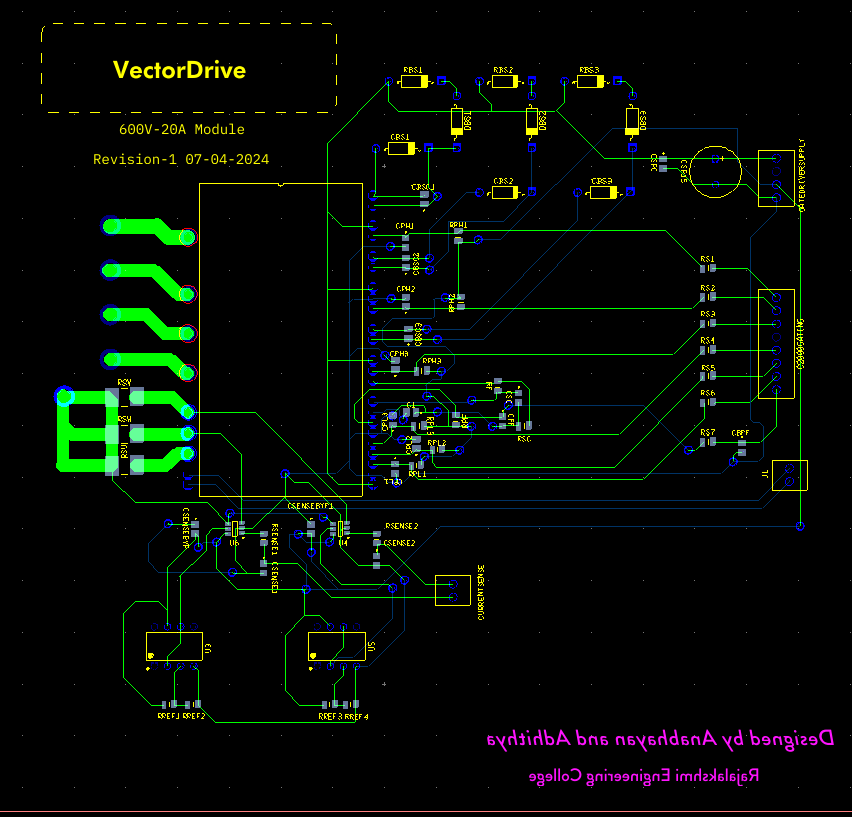
\includegraphics[width=4in]{sections/section4/images/PCBDesign/Ultiboard/Ultiboard.png}}

	\end{figure}
\end{frame}

% Slide 20: 3D View of PCB Layout Design in Ultiboard
\begin{frame}{3D View of PCB Layout}
	\begin{figure}
		\centering

		\fbox{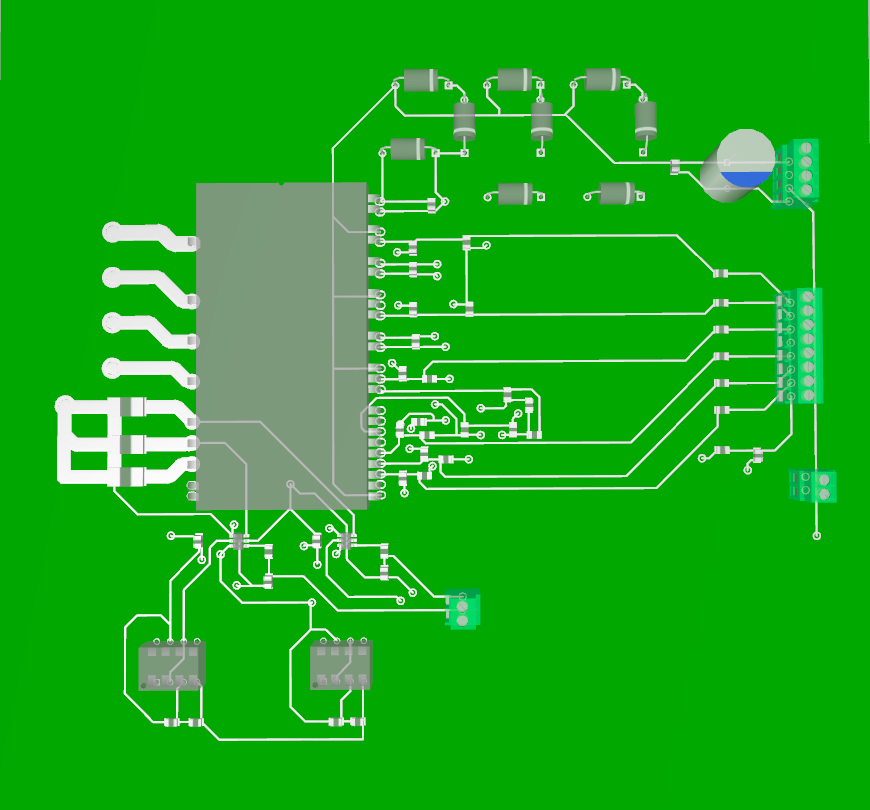
\includegraphics[width=4in]{sections/section4/images/PCBDesign/Ultiboard/3DTopView.png}}

	\end{figure}
\end{frame}

% Slide 21: Current Sensing Circuit in Multisim
\begin{frame}{Current Measurement}
	\begin{figure}
		\centering

		\fbox{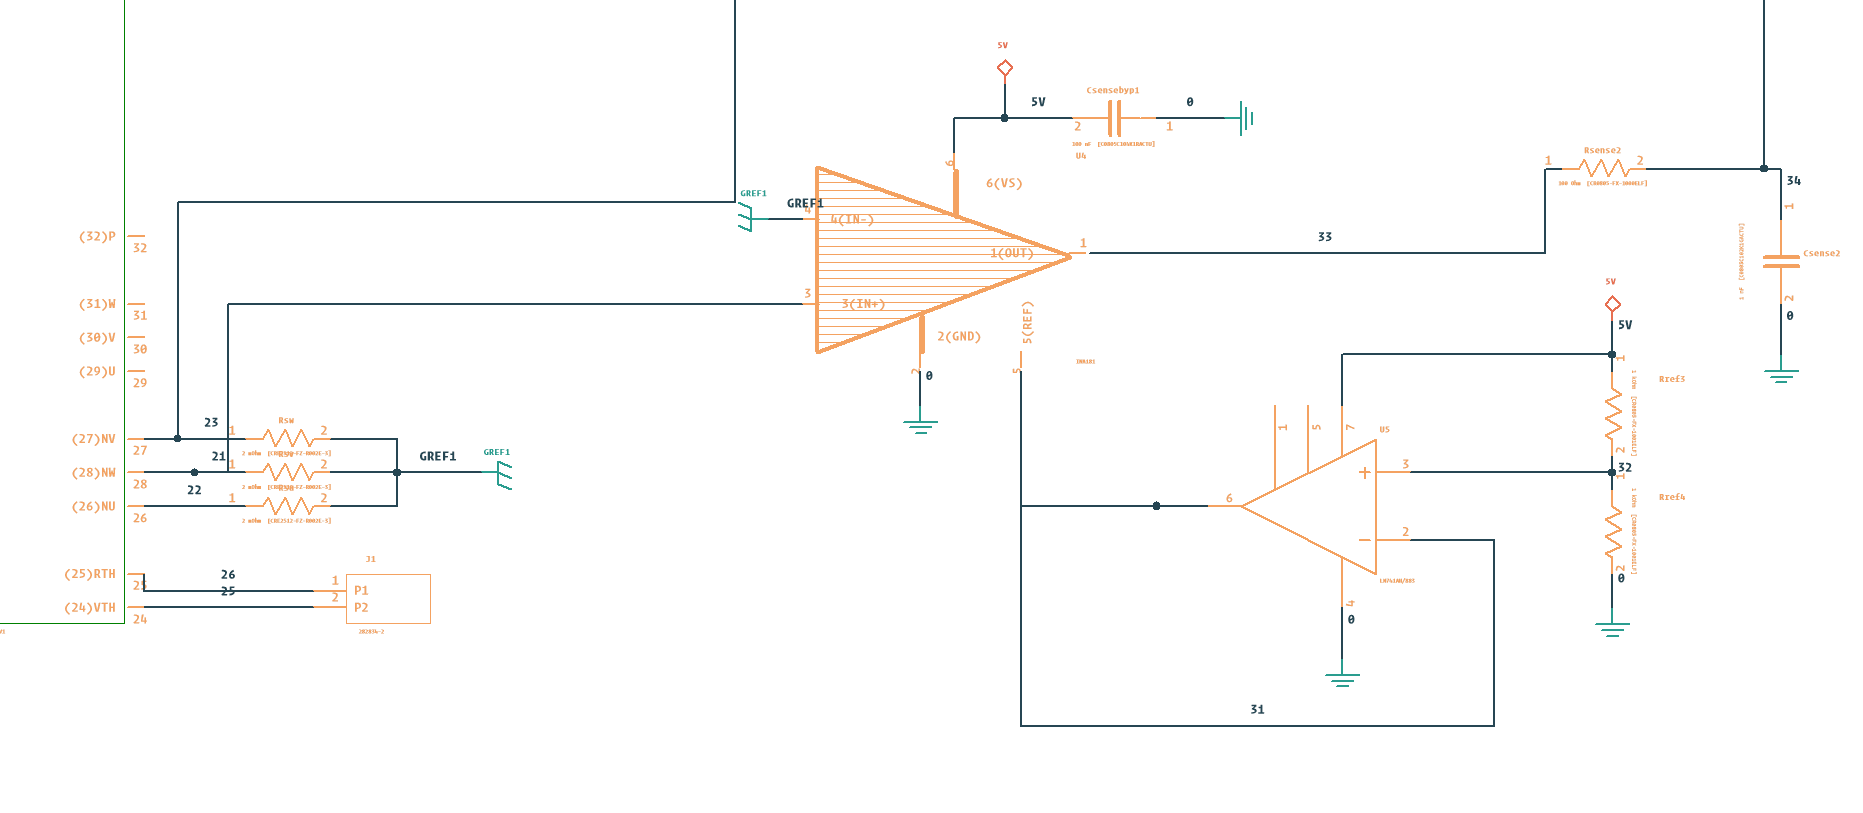
\includegraphics[width=4in]{sections/section4/images/PCBDesign/Multisim/MultisimCurrentSensing.png}}

		\caption{Current Sensing Circuit in Multisim (one phase shown)}
	\end{figure}
\end{frame}

% Slide 22: No-load test setup
\begin{frame}{ACIM Parameter Estimation: No-Load Test}
	\begin{figure}
		\centering

		\fbox{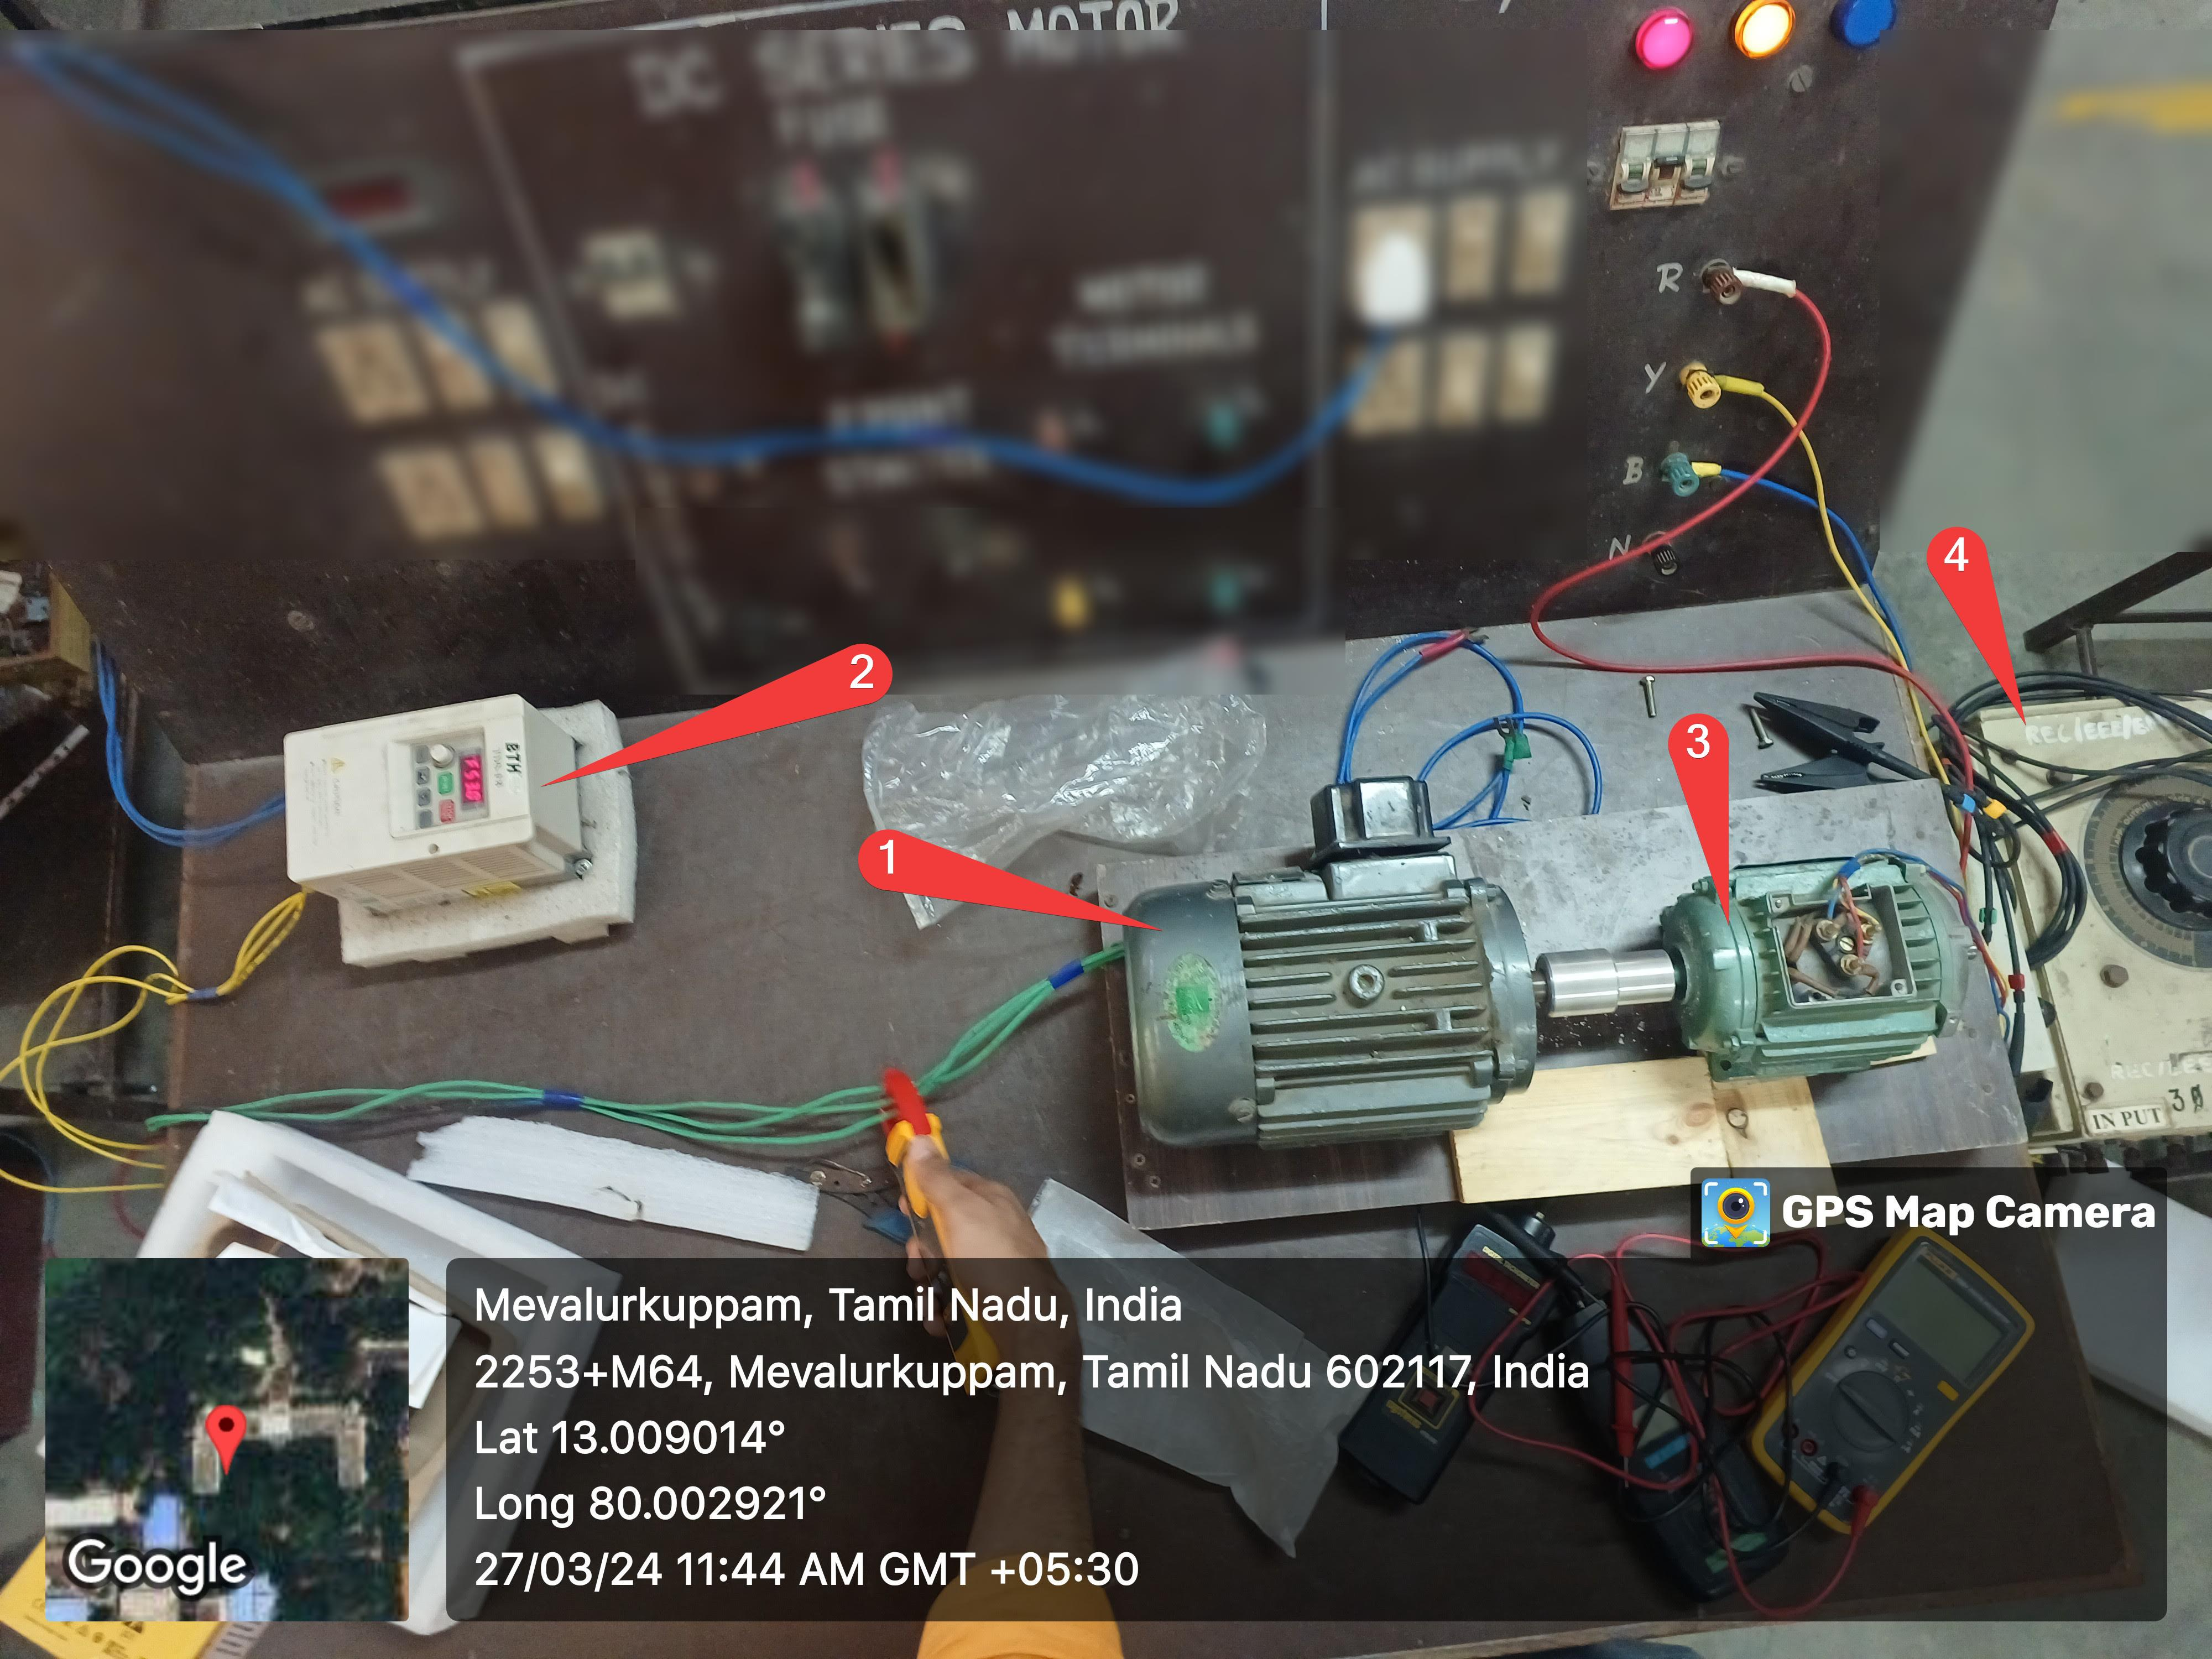
\includegraphics[width=4in]{sections/section5/images/ParamEstim/SetupNoload.jpg}}

		\caption{No-load test setup}
	\end{figure}
\end{frame}

% Slide 23: Fluke 434 power analyzer
\begin{frame}{Fluke 434 Power Analyzer}
	\begin{figure}
		\centering

		\fbox{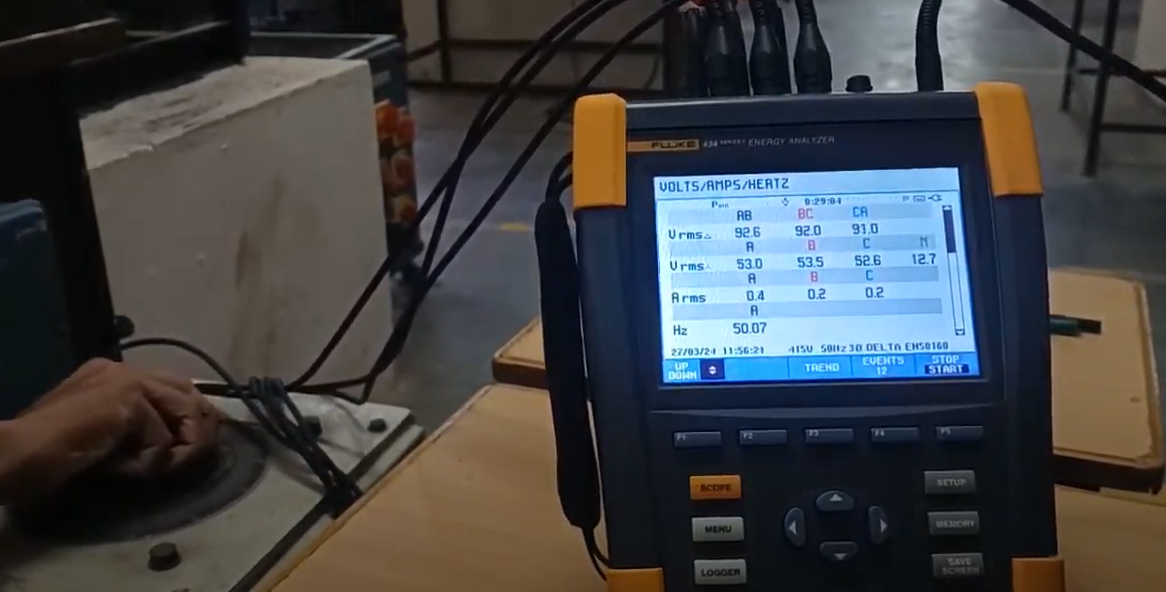
\includegraphics[width=4in]{sections/section5/images/ParamEstim/FlukeVoltAmpHertz.png}}

		\caption{Fluke 434 power analyzer}
	\end{figure}
\end{frame}

% Slide 24: No-load test circuit
\begin{frame}{No-load Test Circuit}
	\begin{figure}
		\centering

		\fbox{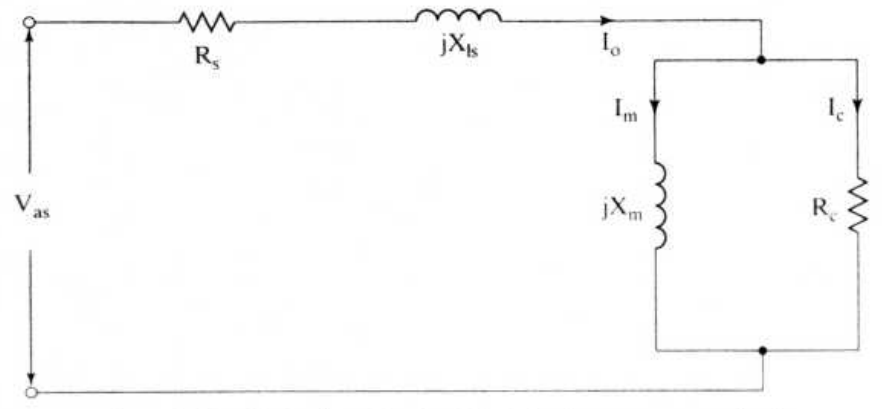
\includegraphics[width=4in]{sections/section5/images/ParamEstim/noloadCircuitKrish.png}}

		\caption{No-load test circuit}
	\end{figure}
\end{frame}

% Slide 25: Blocked rotor test circuit
\begin{frame}{ACIM Parameter Estimation: Blocked Rotor Test}
	\begin{figure}
		\centering

		\fbox{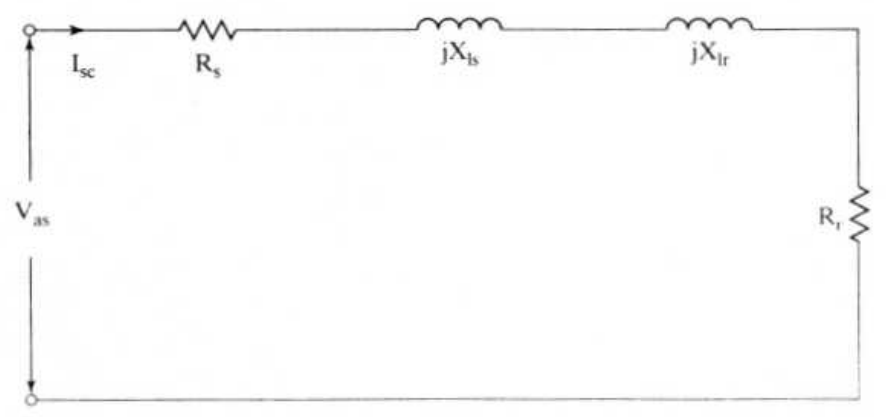
\includegraphics[width=4in]{sections/section5/images/ParamEstim/blockedCircuitKrish.png}}

		\caption{Blocked rotor test circuit}
	\end{figure}
\end{frame}

% Slide 26: ePWM block in Simulink
\begin{frame}{Space Vector Pulse Width Modulation}
	\begin{figure}
		\centering

		\fbox{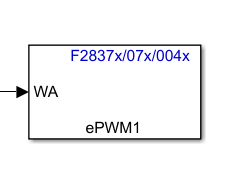
\includegraphics[width=2in]{sections/section6/images/SVPWM/ePWMBlock.png}}

		\caption{ePWM block in Simulink}
	\end{figure}
\end{frame}


% Counter compare and timer period visualtion 1

\begin{frame}{Counter Compare and Timer Period Visualization}
	\begin{figure}
		\centering
		\fbox{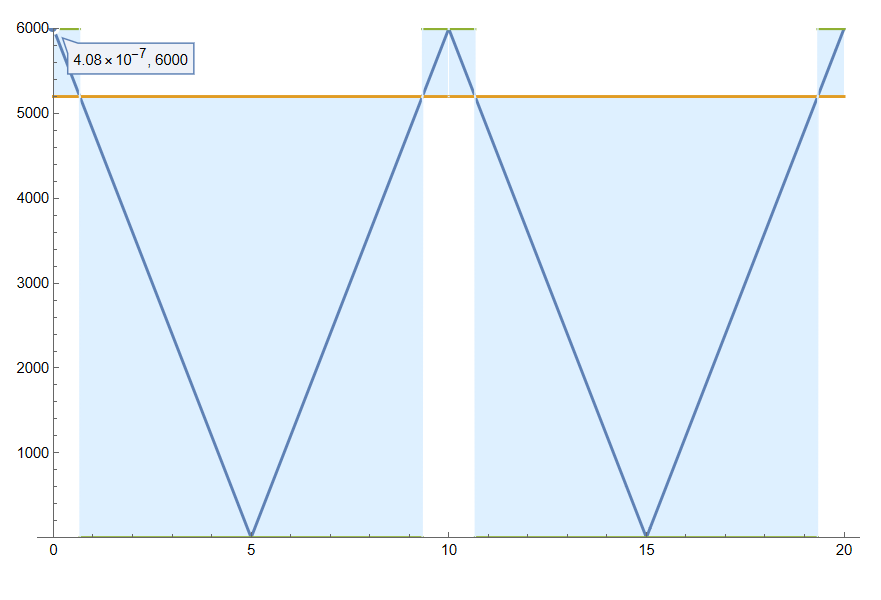
\includegraphics[width=4in]{sections/ppt/CC1.png}}
		\caption{Counter Compare High}
	\end{figure}
\end{frame}

\begin{frame}{Counter Compare and Timer Period Visualization}
	\begin{figure}
		\centering
		\fbox{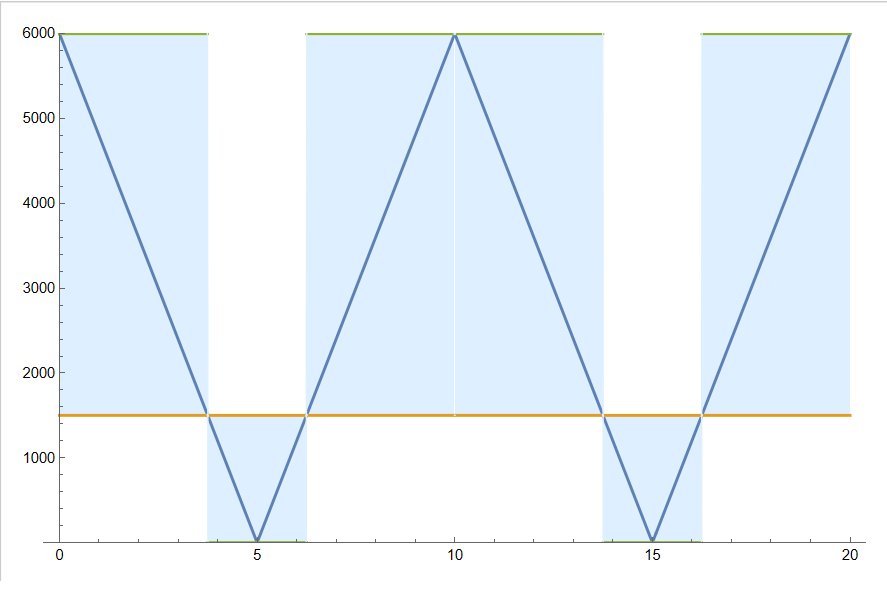
\includegraphics[width=4in]{sections/ppt/CC2.png}}
		\caption{Counter Compare Low}
	\end{figure}
\end{frame}

\begin{frame}{Counter Compare and Timer Period Visualization}
	\begin{figure}
		\centering
		\fbox{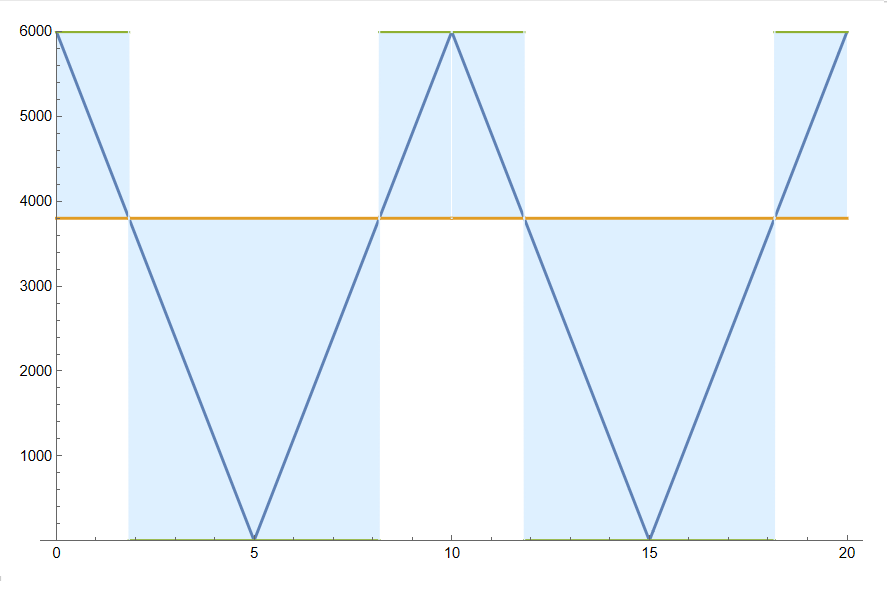
\includegraphics[width=4in]{sections/ppt/CC3.png}}
		\caption{Counter Compare half}
	\end{figure}
\end{frame}


\begin{frame}{TBPRD Calculation}

	\begin{columns}[T]
		\column{0.5\textwidth}
			\begin{itemize}
				\item PWM Frequency ($F_{PWM}$): 15 kHz (recommended by FSAM20SH60A datasheet)
				\item System Clock (SYSCLK): 200 MHz
				\item High Speed Clock Divider (HSPCLKDIV): 1
				\item Clock Divider (CLKDIV): 1
			\end{itemize}
		\column{0.5\textwidth}
			\begin{align*}
				T_{PWM}   & = \frac{1}{F_{PWM}} \\
				T_{TBCLK} & = \frac{SYSCLK}{HSPCLKDIV \times CLKDIV} \\
				TBPRD     & = \frac{T_{PWM}}{2 \times T_{TBCLK}}
			\end{align*}
	\end{columns}

	\vspace{0.5cm}

	\begin{align*}
		T_{PWM}   & = \frac{1}{15 \times 10^3} \text{ seconds} \\
		T_{TBCLK} & = \frac{200 \times 10^6}{1 \times 1} = 200 \times 10^6 \text{ Hz} \\
		TBPRD     & = \frac{\frac{1}{15 \times 10^3}}{2 \times 200 \times 10^6} \approx 6667
	\end{align*}

	\tiny{Therefore, the Timer Period (TBPRD) is 6667.}
\end{frame}


\begin{frame}{ePWM Configuration}
	\begin{figure}
		\centering
		\fbox{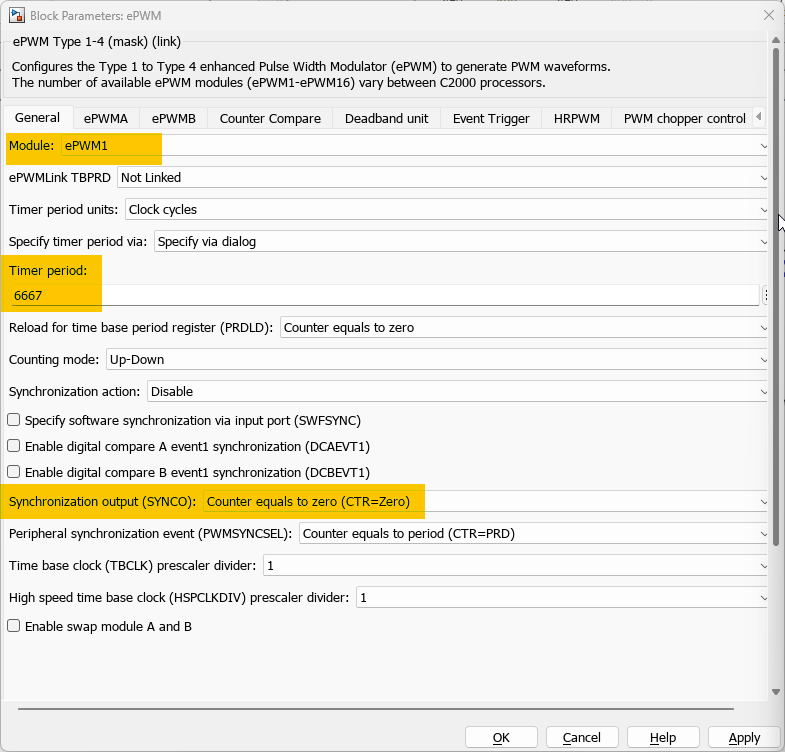
\includegraphics[width=3in]{sections/section6/images/SVPWM/ePWMTBPRD.png}}
		\caption{ePWM configuration in Simulink}
	\end{figure}
\end{frame}
% Slide 28: Hardware setup with RC filter and Launchpad
\begin{frame}{SVPWM with Low Pass Filter}
	\begin{figure}
		\centering

		\fbox{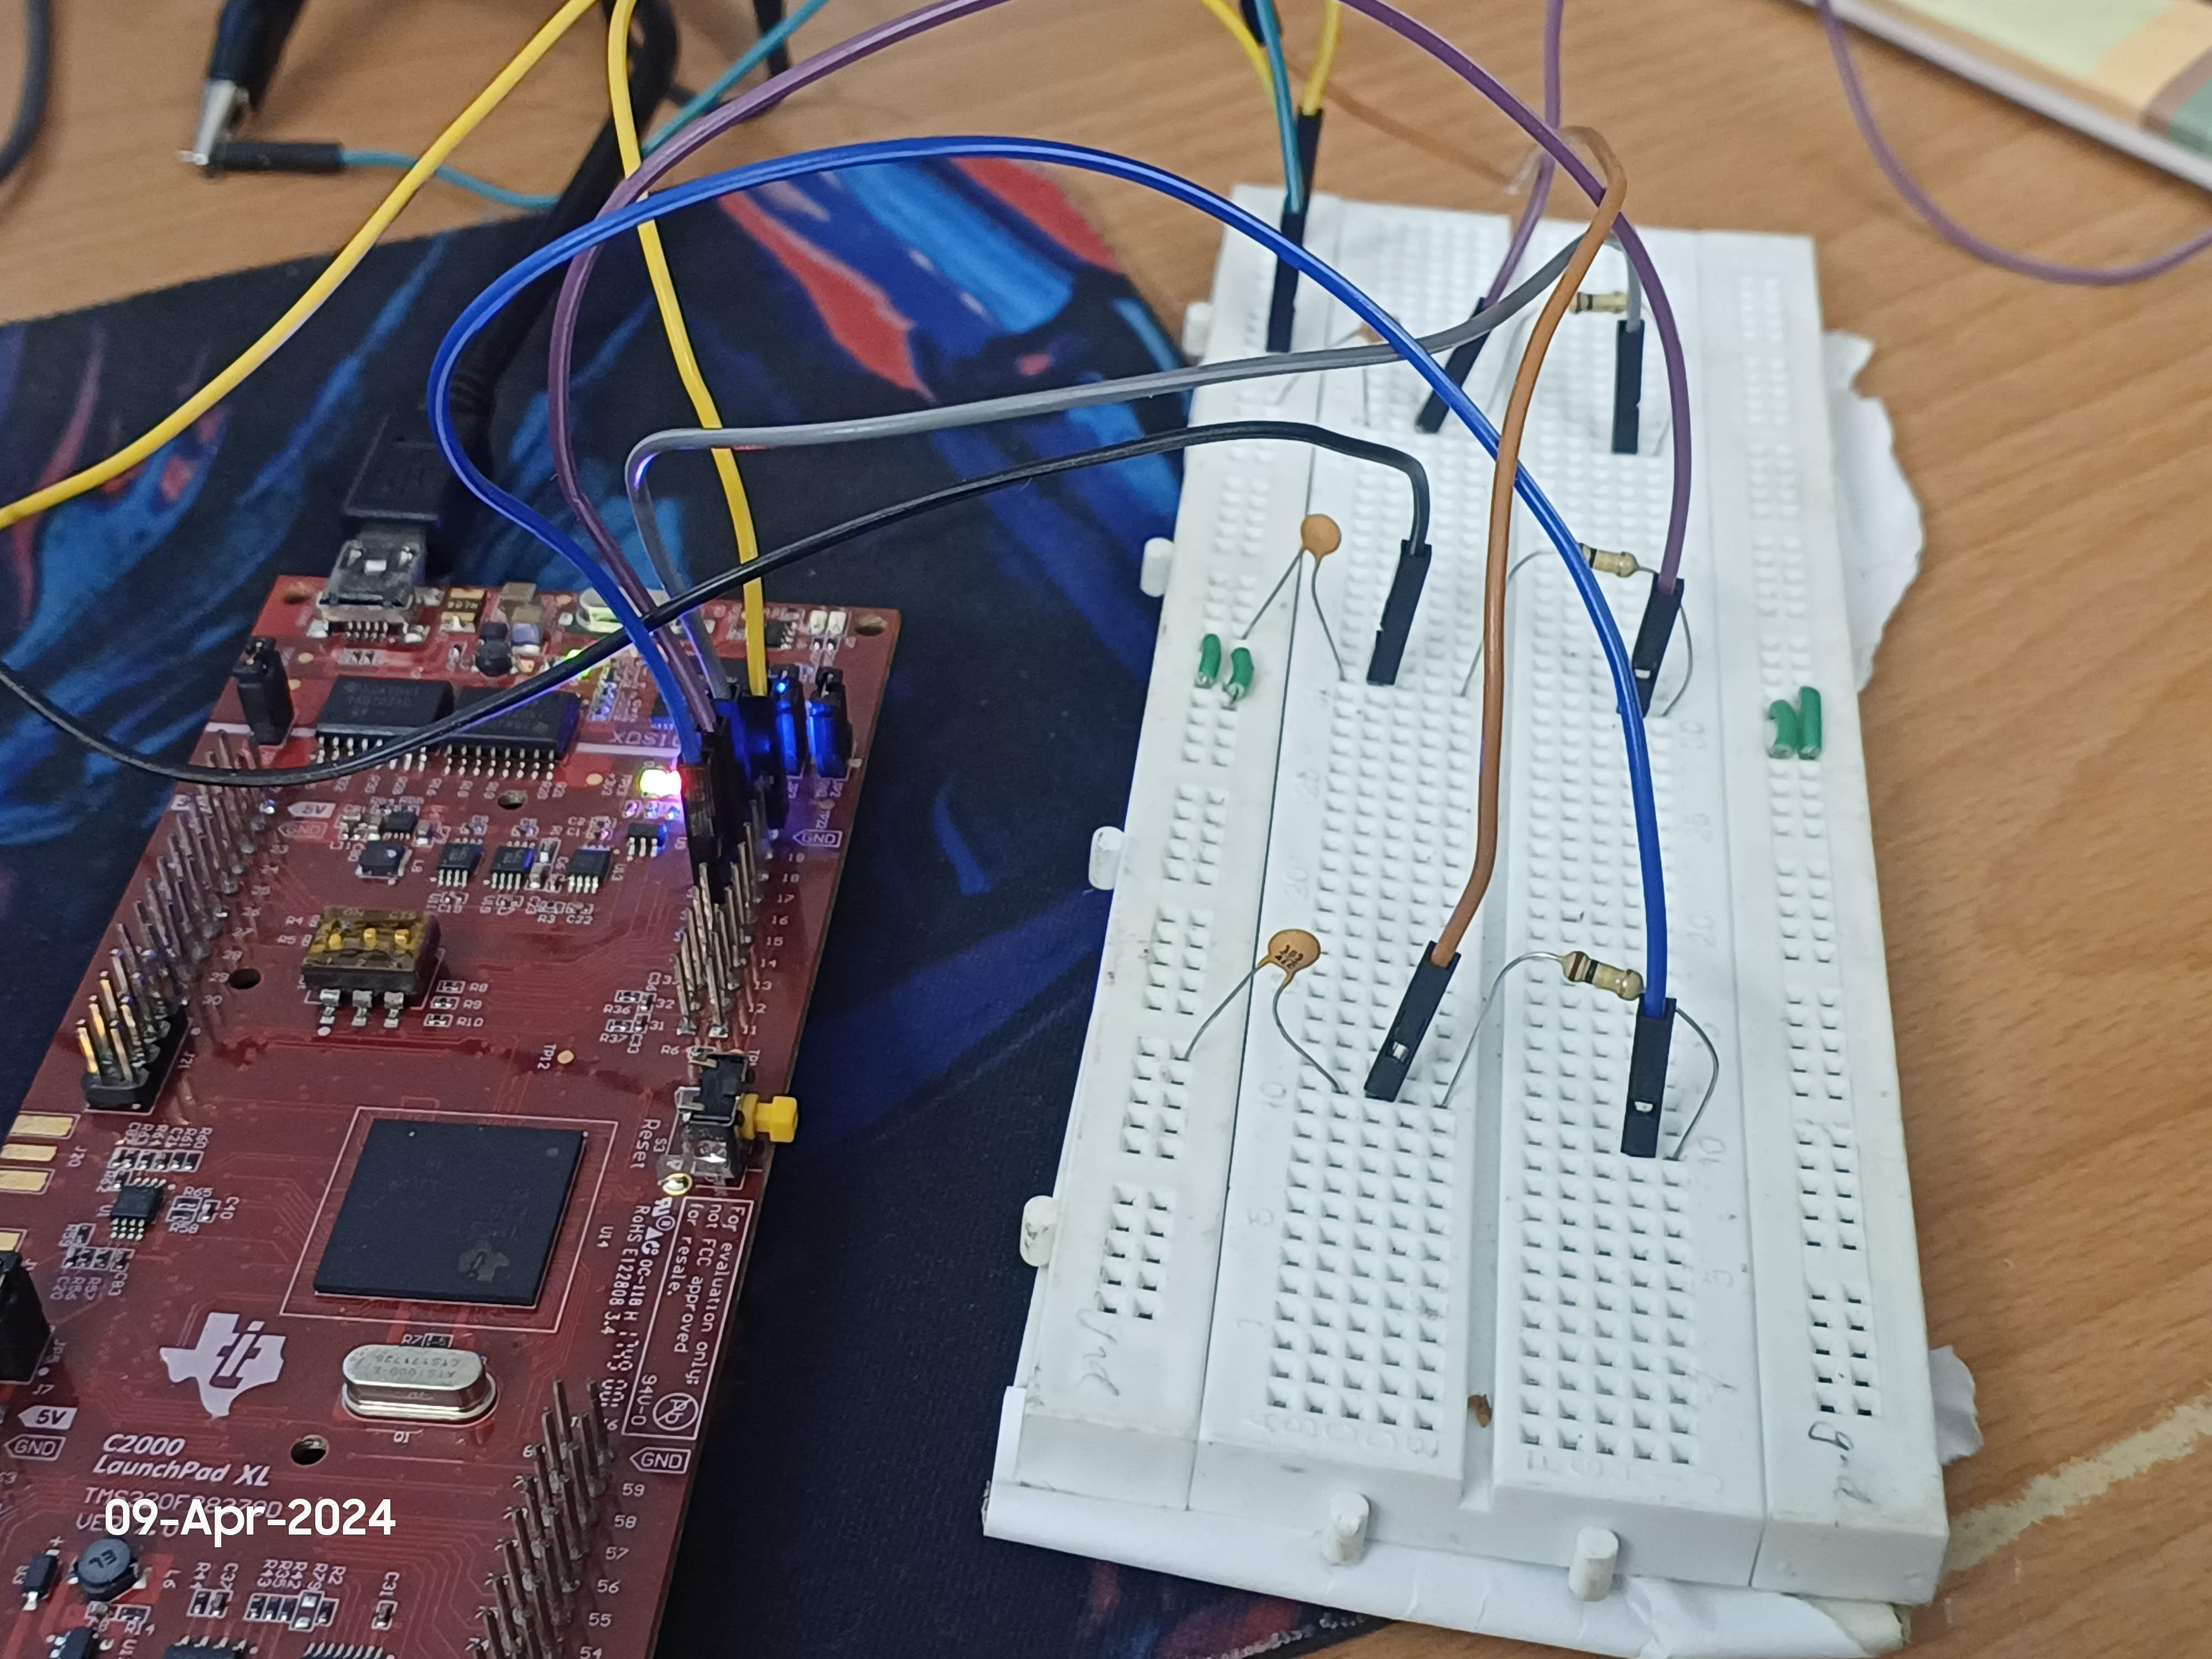
\includegraphics[width=4in]{sections/section6/images/SVPWM/LPFandC2000.jpg}}

		\caption{Hardware setup with RC filter and Launchpad}
	\end{figure}
\end{frame}

% Slide 29: Output of SVPWM with low pass filter
\begin{frame}{Output of SVPWM with LPF}
	\begin{figure}
		\centering

		\fbox{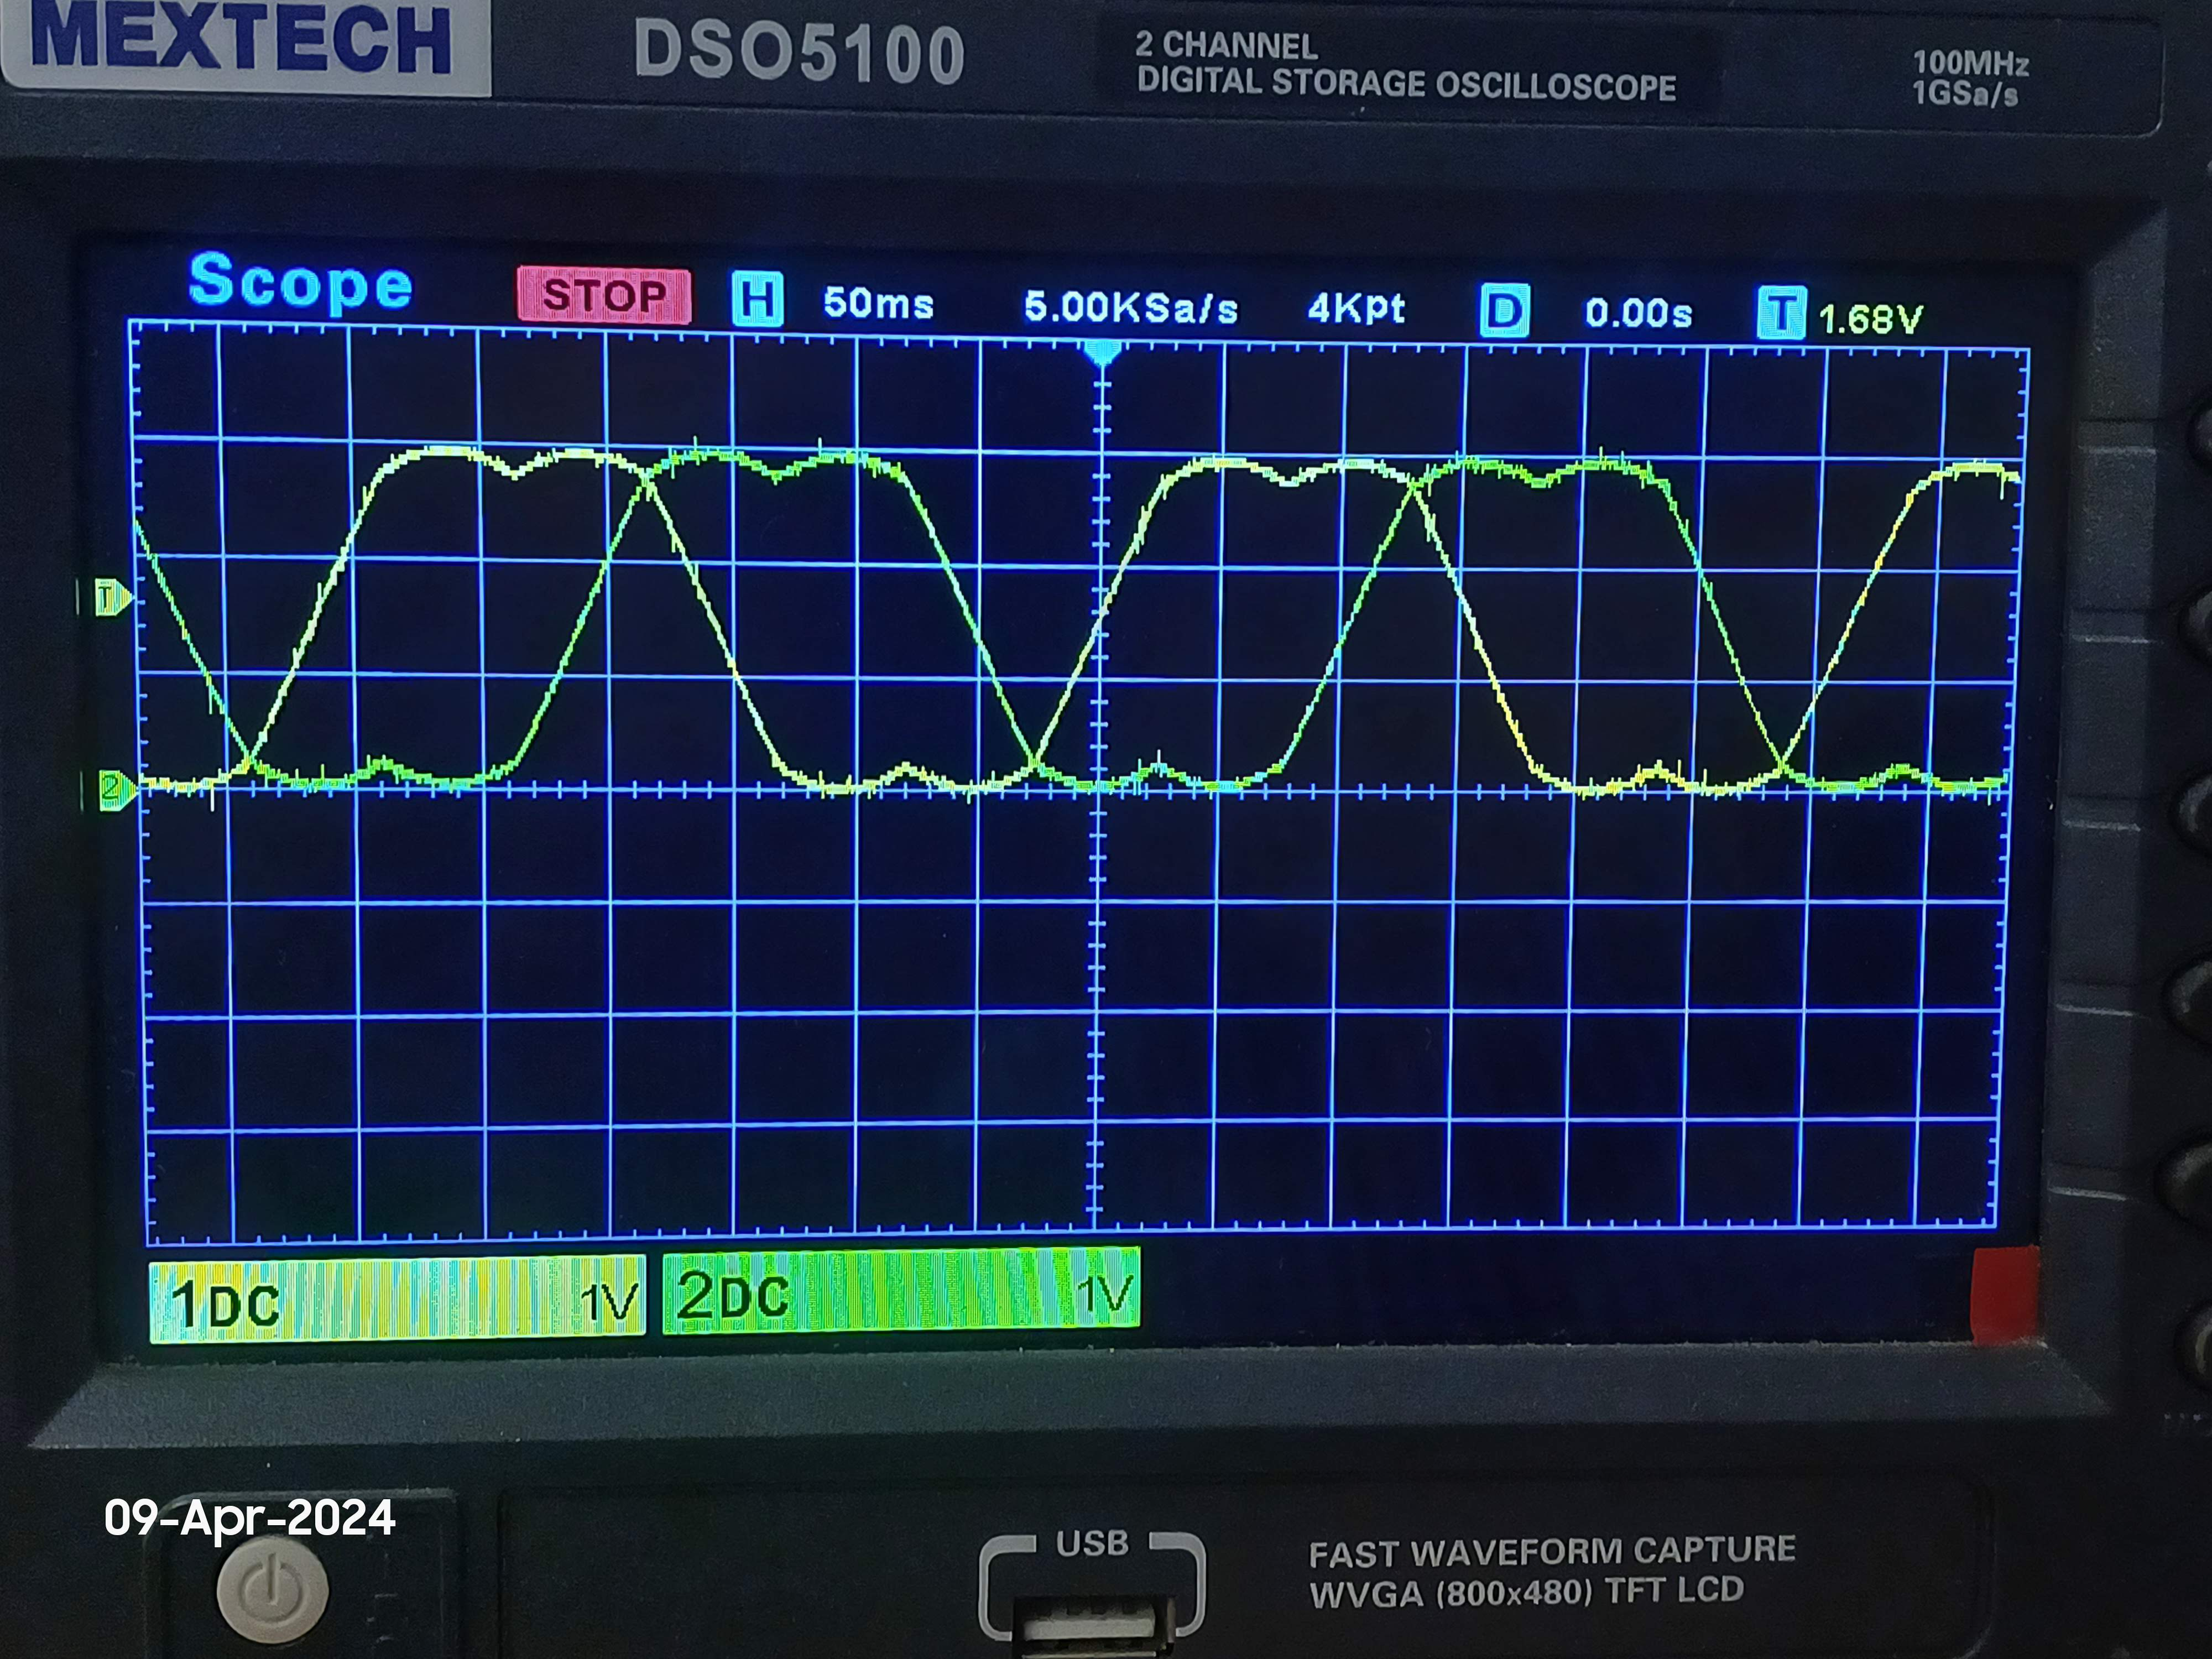
\includegraphics[width=4in]{sections/section6/images/SVPWM/SVPWM2phases.jpg}}

		\caption{Output of SVPWM with low pass filter}
	\end{figure}
\end{frame}

% Slide 30: Dead band time
\begin{frame}{Dead Band Implementation}
	\begin{figure}
		\centering

		\fbox{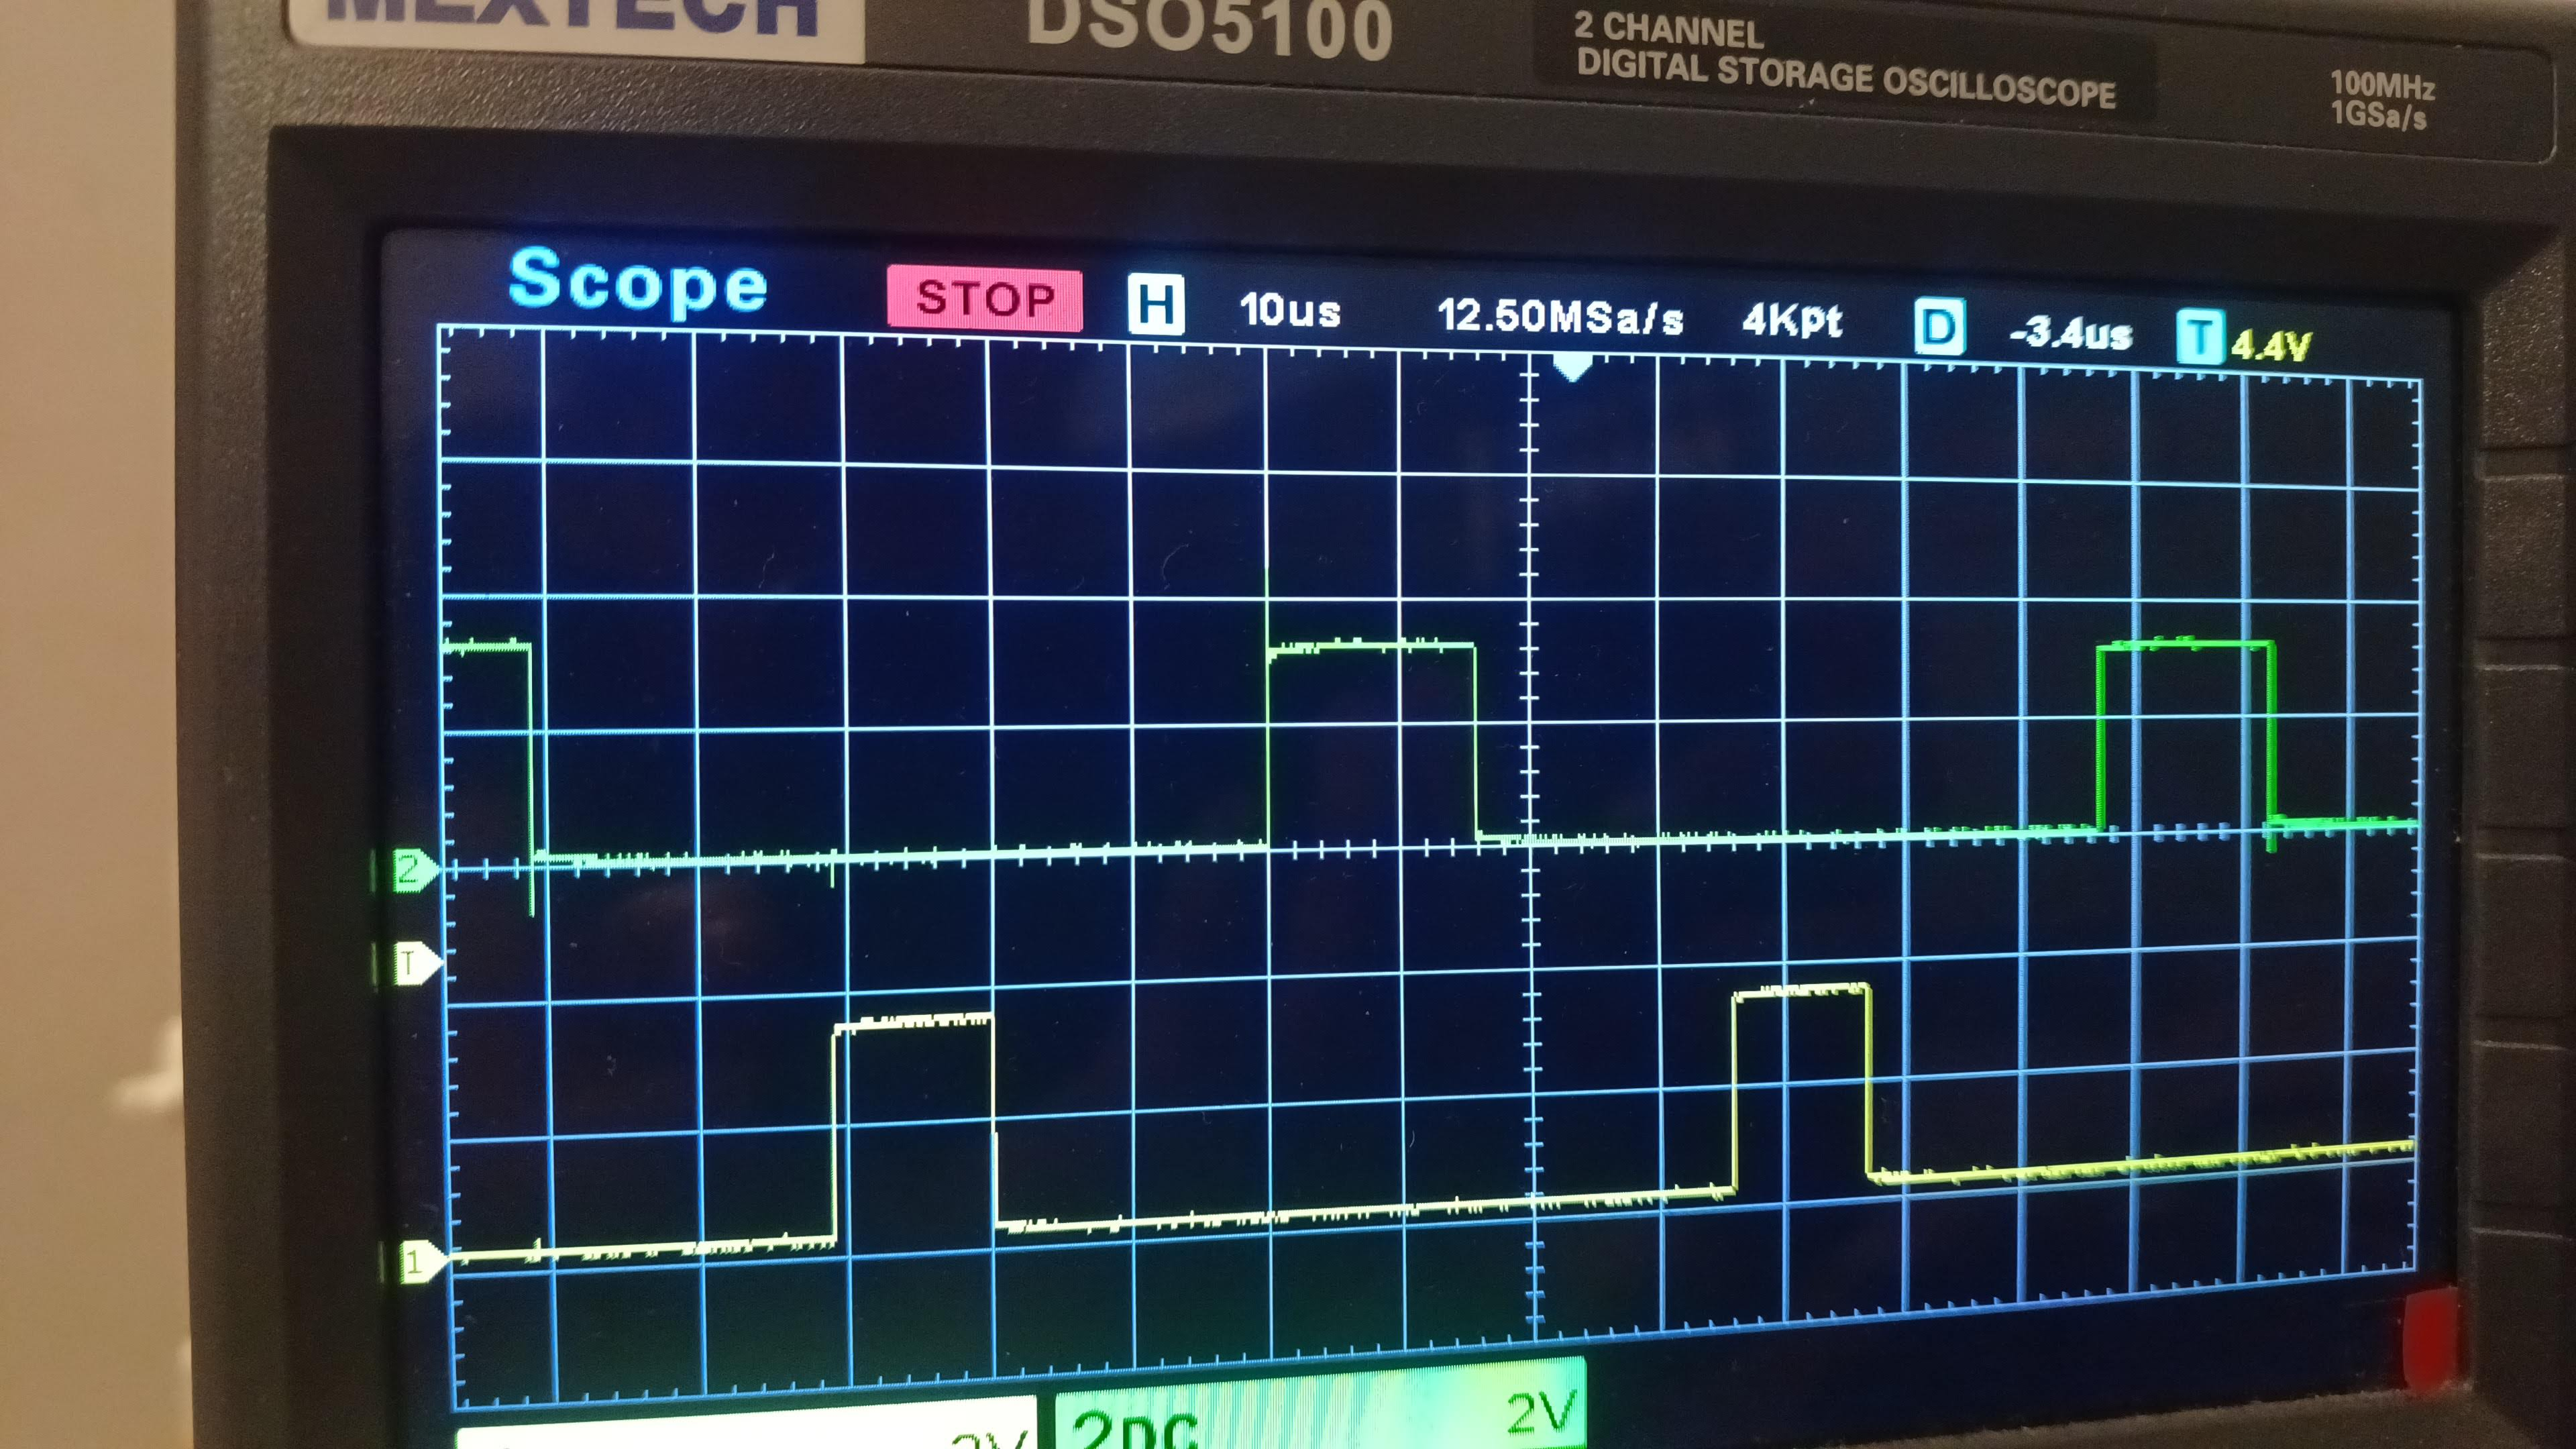
\includegraphics[width=4in]{sections/section6/images/SVPWM/DeadBand20Us.jpeg}}
		\caption{Dead band time}
	\end{figure}
\end{frame}

% Image fbox


\end{document}